\documentclass[paperwidth=48in,paperheight=48in,portrait,final]{baposter}

\usepackage{times}
\usepackage{calc}
\usepackage{graphicx}
\usepackage{amsmath}
\usepackage{amssymb}
\usepackage{relsize}
\usepackage{bm}
\usepackage{listings}
\usepackage{algorithm}
\usepackage{algpseudocode}
\usepackage{float}
\usepackage{multirow,booktabs,ctable,array}
\usepackage{dcolumn}

    \definecolor{listcomment}{rgb}{0.0,0.5,0.0}
    \definecolor{listkeyword}{rgb}{0.0,0.0,0.5}
    \definecolor{listnumbers}{gray}{0.65}
    \definecolor{listlightgray}{gray}{0.955}
    \definecolor{listwhite}{gray}{1.0}


\newcolumntype{d}[1]{D{.}{.}{-1} }

\lstset{frame = htb,
        framerule = 0.25pt,
        float,
        fontadjust,
        backgroundcolor={\color{listlightgray}},
        basicstyle = {\ttfamily\scriptsize},
        keywordstyle = {\ttfamily\color{listkeyword}},
        identifierstyle = {\ttfamily},
        commentstyle = {\ttfamily\color{listcomment}},
        stringstyle = {\ttfamily},
        showstringspaces = false,
        showtabs = false,
        numbers = none,
        numbersep = 6pt,
        numberstyle={\ttfamily\color{listnumbers}},
        tabsize = 2,
        language=bash,
        floatplacement=!h,
        caption={},
        captionpos=b,
        label=listing:antsRegistration
        }


\usepackage{graphicx}
\usepackage{multicol}

\usepackage{pgfbaselayers}
\pgfdeclarelayer{background}
\pgfdeclarelayer{foreground}
\pgfsetlayers{background,main,foreground}

\usepackage{helvet}
\usepackage{bookman}
\usepackage{palatino}

\newcommand{\captionfont}{\footnotesize}

\selectcolormodel{cmyk}

\graphicspath{{images/}}

%%%%%%%%%%%%%%%%%%%%%%%%%%%%%%%%%%%%%%%%%%%%%%%%%%%%%%%%%%%%%%%%%%%%%%%%%%%%%%%%
%%%% Some math symbols used in the text
%%%%%%%%%%%%%%%%%%%%%%%%%%%%%%%%%%%%%%%%%%%%%%%%%%%%%%%%%%%%%%%%%%%%%%%%%%%%%%%%
% Format 
\newcommand{\Matrix}[1]{\begin{bmatrix} #1 \end{bmatrix}}
\newcommand{\Vector}[1]{\Matrix{#1}}
\newcommand*{\SET}[1]  {\ensuremath{\mathcal{#1}}}
\newcommand*{\MAT}[1]  {\ensuremath{\mathbf{#1}}}
\newcommand*{\VEC}[1]  {\ensuremath{\bm{#1}}}
\newcommand*{\CONST}[1]{\ensuremath{\mathit{#1}}}
\newcommand*{\norm}[1]{\mathopen\| #1 \mathclose\|}% use instead of $\|x\|$
\newcommand*{\abs}[1]{\mathopen| #1 \mathclose|}% use instead of $\|x\|$
\newcommand*{\absLR}[1]{\left| #1 \right|}% use instead of $\|x\|$

\def\norm#1{\mathopen\| #1 \mathclose\|}% use instead of $\|x\|$
\newcommand{\normLR}[1]{\left\| #1 \right\|}% use instead of $\|x\|$

%%%%%%%%%%%%%%%%%%%%%%%%%%%%%%%%%%%%%%%%%%%%%%%%%%%%%%%%%%%%%%%%%%%%%%%%%%%%%%%%
% Multicol Settings
%%%%%%%%%%%%%%%%%%%%%%%%%%%%%%%%%%%%%%%%%%%%%%%%%%%%%%%%%%%%%%%%%%%%%%%%%%%%%%%%
\setlength{\columnsep}{0.7em}
\setlength{\columnseprule}{0mm}


%%%%%%%%%%%%%%%%%%%%%%%%%%%%%%%%%%%%%%%%%%%%%%%%%%%%%%%%%%%%%%%%%%%%%%%%%%%%%%%%
% Save space in lists. Use this after the opening of the list
%%%%%%%%%%%%%%%%%%%%%%%%%%%%%%%%%%%%%%%%%%%%%%%%%%%%%%%%%%%%%%%%%%%%%%%%%%%%%%%%
\newcommand{\compresslist}{%
\setlength{\itemsep}{1pt}%
\setlength{\parskip}{0pt}%
\setlength{\parsep}{0pt}%
}


%%%%%%%%%%%%%%%%%%%%%%%%%%%%%%%%%%%%%%%%%%%%%%%%%%%%%%%%%%%%%%%%%%%%%%%%%%%%%%
%%% Begin of Document
%%%%%%%%%%%%%%%%%%%%%%%%%%%%%%%%%%%%%%%%%%%%%%%%%%%%%%%%%%%%%%%%%%%%%%%%%%%%%%

\begin{document}

%%%%%%%%%%%%%%%%%%%%%%%%%%%%%%%%%%%%%%%%%%%%%%%%%%%%%%%%%%%%%%%%%%%%%%%%%%%%%%
%%% Here starts the poster
%%%---------------------------------------------------------------------------
%%% Format it to your taste with the options
%%%%%%%%%%%%%%%%%%%%%%%%%%%%%%%%%%%%%%%%%%%%%%%%%%%%%%%%%%%%%%%%%%%%%%%%%%%%%%
\typeout{Poster Starts}
\background{
  \begin{tikzpicture}[remember picture,overlay]%
    \draw (current page.north west)+(-2em,-0em) node[anchor=north west] {\hspace{-2em}\includegraphics[height=1.1\textheight]{silhouettes_background}};
  \end{tikzpicture}%
}
\definecolor{silver}{cmyk}{0,0,0,0.3}
\definecolor{yellow}{cmyk}{0,0,0.9,0.0}
\definecolor{reddishyellow}{cmyk}{0,0.22,1.0,0.0}
\definecolor{black}{cmyk}{0,0,0.0,1.0}
\definecolor{darkYellow}{cmyk}{0,0,1.0,0.5}
\definecolor{darkSilver}{cmyk}{0,0,0,0.1}

\definecolor{lightyellow}{cmyk}{0,0,0.3,0.0}
\definecolor{lighteryellow}{cmyk}{0,0,0.1,0.0}
\definecolor{lightestyellow}{cmyk}{0,0,0.05,0.0}

% http://www.creativecolorschemes.com/resources/free-color-schemes/blue-tone-color-scheme.shtml

\definecolor{colorA}{cmyk}{1,0.25,0.1,0.5}
\definecolor{colorB}{cmyk}{1,0.3,0.05,0.2}
\definecolor{colorC}{cmyk}{0.6,0,0.05,0}
\definecolor{colorD}{cmyk}{0.95,0.6,0.05,0.15}
\definecolor{colorE}{cmyk}{0.6,0.3,0.05,0.05}
\definecolor{colorF}{cmyk}{0.4,0.15,0,0}
\definecolor{colorf}{cmyk}{0.1,0.0375,0,0}
\definecolor{colorG}{cmyk}{0.75,0.3,0.05,0.1}
\definecolor{colorH}{cmyk}{0.65,0.15,0,0.05}
\definecolor{colorI}{cmyk}{0.3,0.05,0,0}
\definecolor{colorJ}{cmyk}{0.65,0,1,0}
\definecolor{colorK}{cmyk}{0,0.5,1,0}
\definecolor{colork}{cmyk}{0,0.125,0.25,0}
\definecolor{colorL}{cmyk}{0.65,0.8,0,0}
\definecolor{colorM}{cmyk}{0.7,0.4,0.2,0.6}
\definecolor{colorN}{cmyk}{0.3,0.15,0.1,0.3}
\definecolor{colorn}{cmyk}{0.075,0.0375,0.025,0.075}
\definecolor{colorO}{cmyk}{0.25,0.05,0.1,0.15}

%%
\typeout{Poster Starts}
\background{
	\begin{tikzpicture}[remember picture,overlay]%
	\draw (current page.north west)+(-2em,2em) node[anchor=north west]
	{\includegraphics[height=1.1\textheight]{background}};
	\end{tikzpicture}
}

\begin{poster}%
  % Poster Options
  {
  % Show grid to help with alignment
  grid=false,
  % Column spacing
  colspacing=1em,
  % Color style
  bgColorOne=colorf,
  bgColorTwo=white,
  borderColor=colorK,
  headerColorOne=colork,
  headerColorTwo=white,
  headerFontColor=colorM,
  boxColorOne=white,
  boxColorTwo=colorC,
  % Format of textbox
  textborder=roundedleft,
%  textborder=rectangle,
  % Format of text header
  eyecatcher=false,
  headerborder=open,
  headerheight=0.1\textheight,
  headershape=roundedright,
  headershade=plain,
  headerfont=\Large\textsf, %Sans Serif
  boxshade=plain,
%  background=shade-tb,
  background=plain,
  linewidth=2pt
  }
  % Eye Catcher
  {} % No eye catcher for this poster. If an eye catcher is present, the title is centered between eye-catcher and logo.
  % Title
  {%Sans Serif
  %\bf% Serif
  Advanced Normalization Tools for Cardiac Motion Correction
  \vspace{5mm}
  }
  % Authors
  { %Sans Serif
  % Serif
  Nicholas J. Tustison, Yang Yang, Michael Salerno\newline
  {\smaller University of Virginia, Charlottesville, VA, USA}
  }
  % University logo
  { 
  
\includegraphics[height=6em]{uvalogo}
  }

  \tikzstyle{light shaded}=[top color=baposterBGtwo!30!white,bottom color=baposterBGone!30!white,shading=axis,shading angle=30]

  % Width of left inset image
     \newlength{\leftimgwidth}
     \setlength{\leftimgwidth}{0.78em+8.0em}



%%%%%%%%%%%%%%%%%%%%%%%%%%%%%%%%%%%%%%%%%%%%%%%%%%%%%%%%%%%%%%%%%%%%%%%%%%%%%%
%%% Now define the boxes that make up the poster
%%%---------------------------------------------------------------------------
%%% Each box has a name and can be placed absolutely or relatively.
%%% The only inconvenience is that you can only specify a relative position 
%%% towards an already declared box. So if you have a box attached to the 
%%% bottom, one to the top and a third one which should be in between, you 
%%% have to specify the top and bottom boxes before you specify the middle 
%%% box.
%%%%%%%%%%%%%%%%%%%%%%%%%%%%%%%%%%%%%%%%%%%%%%%%%%%%%%%%%%%%%%%%%%%%%%%%%%%%%%

%%%%%%%%%%%%%%%%%%%%%%%%%%%%%%%%%%%%%%%%%%%%%%%%%%%%%%%%%%%%%%%%%%%%%%%%%%%%%%
  \headerbox{Introduction}{name=introduction,column=0,row=0}{
%%%%%%%%%%%%%%%%%%%%%%%%%%%%%%%%%%%%%%%%%%%%%%%%%%%%%%%%%%%%%%%%%%%%%%%%%%%%%%
  \vspace{0.3em}

Motion correction for dynamic contrast MR myocardial perfusion is of significant 
research interest and has resulted in several techniques generally characterized 
as rigid or non-rigid image registration-based. To bring together interested 
researchers for discussion and comparison of methods for correction of motion 
artefacts and the development of performance benchmarks of such techniques, the 
Statistical Atlases and Computational Modeling of the Heart (STACOM) workshop 
committee organized a motion correction challenge to be held in conjunction with 
international 2014 conference of the Medical Image Computing and Computer Assisted 
Intervention (MICCAI) Society.

  \vspace{0.3em}
 }

%%%%%%%%%%%%%%%%%%%%%%%%%%%%%%%%%%%%%%%%%%%%%%%%%%%%%%%%%%%%%%%%%%%%%%%%%%%%%%
  \headerbox{Data}{name=data,column=0,below=introduction}{
%%%%%%%%%%%%%%%%%%%%%%%%%%%%%%%%%%%%%%%%%%%%%%%%%%%%%%%%%%%%%%%%%%%%%%%%%%%%%%
  \vspace{0.3em}

For comparative evaluation, each team was given MR perfusion 
data described by the organizers:
\begin{quote}
The evaluation dataset consists of 10 cases from two centres: the University of Utah and University of Auckland. For each case, a single short axis slice time series at rest and at stress is provided. The Utah datasets were acquired using a saturation-recovery radial turboFLASH sequence at rest and during adenosine infusion (140 $\mu$g/kg/min), as described in \cite{dibella2012}. Contrast was 5 cc/s injection of Multihance (Gd-BOPTA) at 0.02 mmol/kg for the rest and 0.03 mmol/kg for the stress. Four of these subjects have known coronary artery disease. The Auckland cases were acquired using a saturation-recovery Cartesian turboFLASH sequence at rest and during adenosine infusion (140 $\mu$g/kg/min). Contrast was 0.04 mmol/kg Omniscan (gadodiamide). None of the Auckland cases have overt coronary disease. Expert-drawn contours only at a reference frame, chosen when contrast is present in both ventricles, were provided to the participants.
\end{quote}

      \vspace{0.3em}
  }

%%%%%%%%%%%%%%%%%%%%%%%%%%%%%%%%%%%%%%%%%%%%%%%%%%%%%%%%%%%%%%%%%%%%%%%%%%%%%%
  \headerbox{Preprocessing}{name=preprocessing,column=0,below=data,above=bottom}{
%%%%%%%%%%%%%%%%%%%%%%%%%%%%%%%%%%%%%%%%%%%%%%%%%%%%%%%%%%%%%%%%%%%%%%%%%%%%%%
  \vspace{0.3em}

Given the temporal image variability and other confounds (e.g., noise), a multivariate 
image registration strategy was employed made possible by recent developmental work 
to the Insight Toolkit \cite{avants2014}.  This strategy involved the following three
derived images:
\begin{itemize}
  \item N4 bias corrected \cite{tustison2010},
  \item noise-filtered, structure-preserving SUSAN image \cite{smith1997}, and
  \item low level Laplacian-based edge detection.
\end{itemize}

Sample preprocessed images used:

\begin{center}
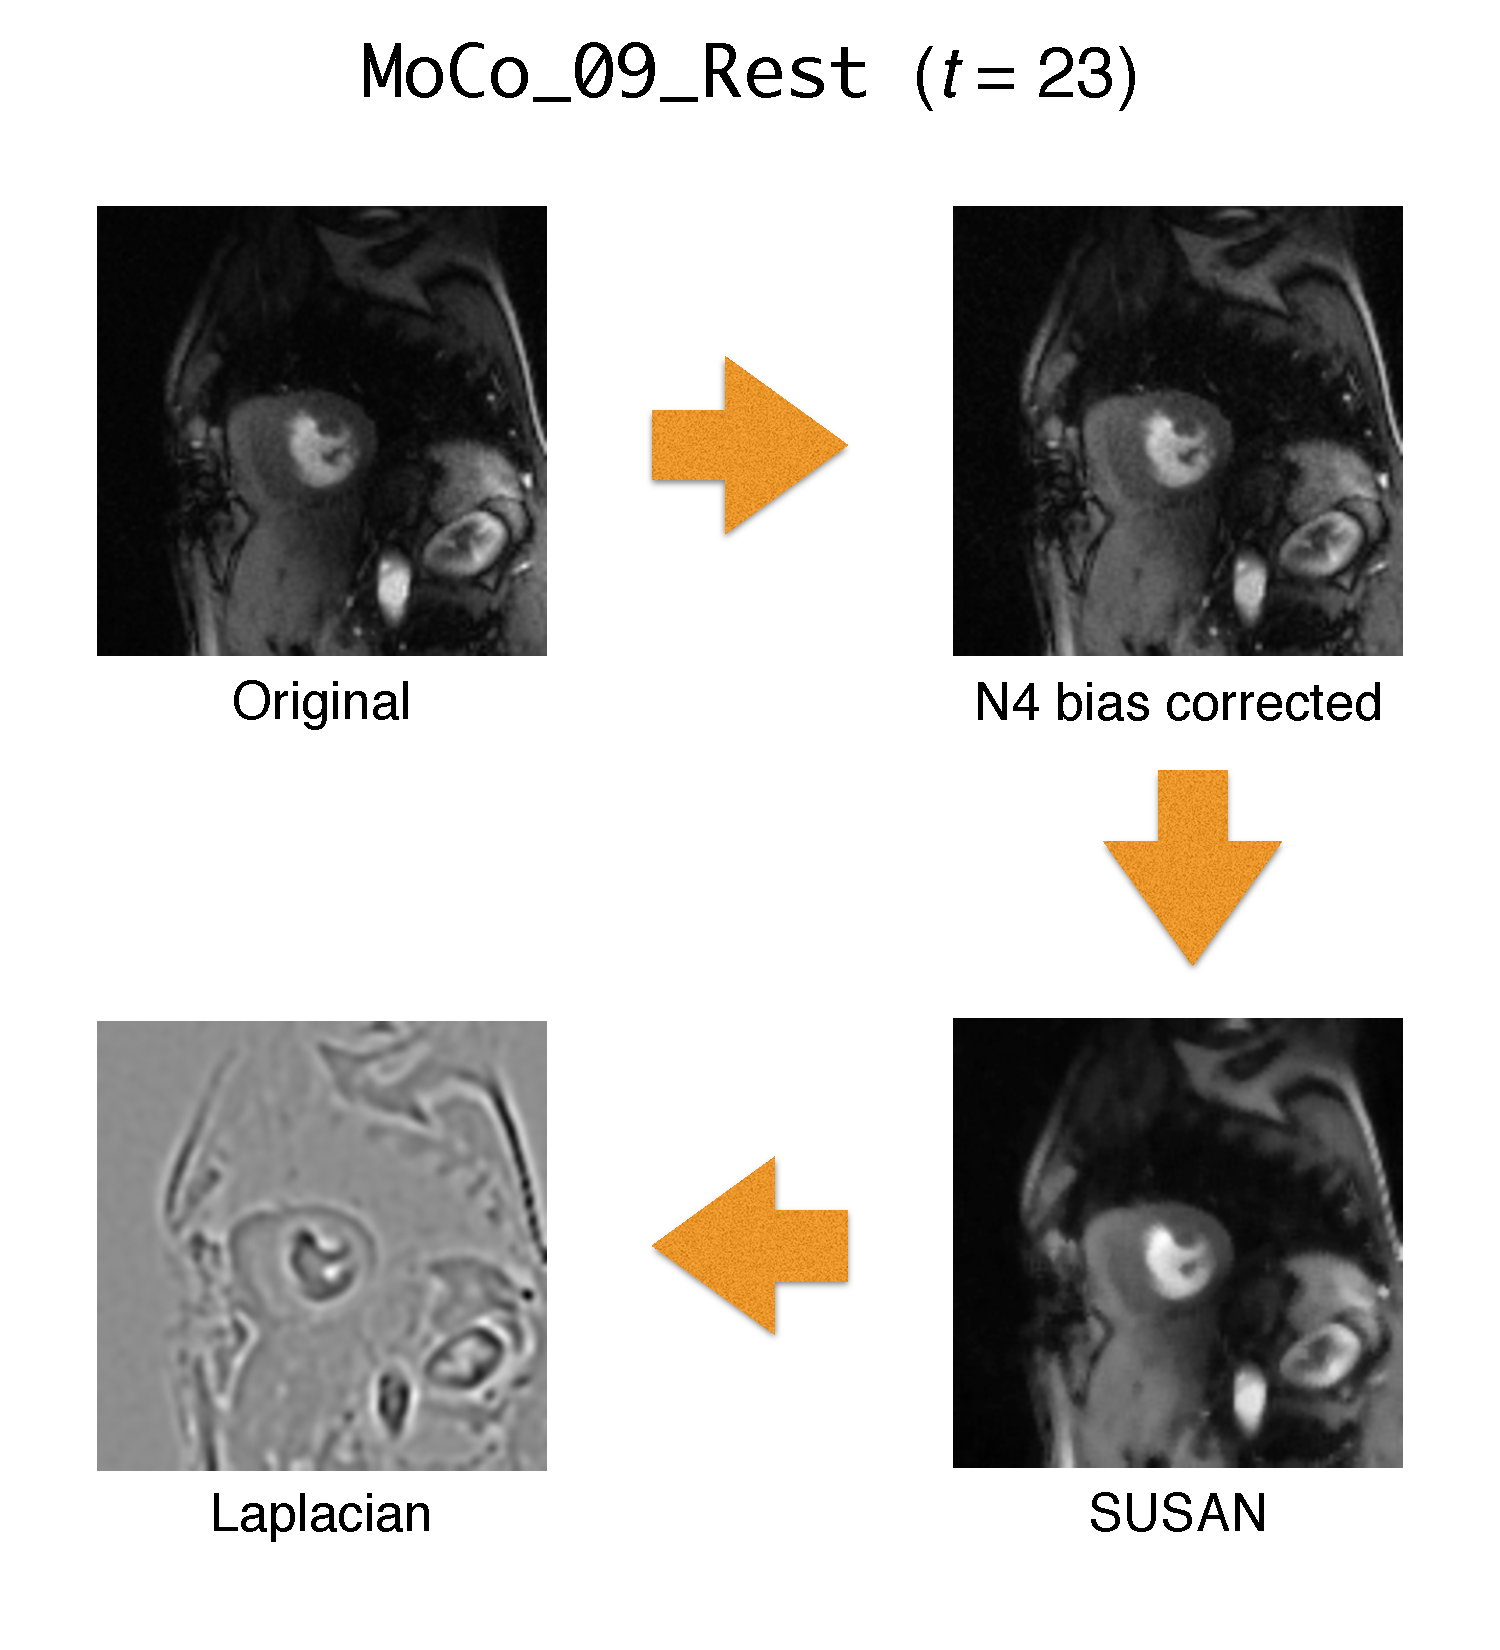
\includegraphics[width=85mm]{../Figures/MoCo_09_Rest_23.pdf}
\end{center}

  \vspace{0.3em}
  }

%%%%%%%%%%%%%%%%%%%%%%%%%%%%%%%%%%%%%%%%%%%%%%%%%%%%%%%%%%%%%%%%%%%%%%%%%%%%%%
  \headerbox{B-Spline SyN Multivariate Image Registration}{name=bsyn,column=1,span=1}{
%%%%%%%%%%%%%%%%%%%%%%%%%%%%%%%%%%%%%%%%%%%%%%%%%%%%%%%%%%%%%%%%%%%%%%%%%%%%%%
\vspace{0.3em}

{\bf Theory}
\vspace{0.5em} 

The Symmetric Normalization (SyN) diffeomorphic approach \cite{avants2008} to pairwise image 
registration minimizes the following symmetric formulation:
\begin{align}
\label{eq:syn}
  \inf_{\phi_1} \inf_{\phi_2}   \Bigg[
                     \int_0^{0.5} & \left( \|v_1(t)\|_L^2 + \|v_2(t)\|_L^2 \right) dt \nonumber \\
                     &+
                     \int_{\Omega} \Pi_{\sim}
                          \left( I \circ \phi_1^{-1}(\mathbf{x},0.5),
                           J \circ \phi_2^{-1}(\mathbf{x},0.5) \right) d\Omega \Bigg]
\end{align}
where
\begin{align}
  \frac{d \phi_i(\mathbf{x},t)}{dt} = v_i( \phi_i(\mathbf{x},t), t ),\,\, \phi_i(\mathbf{x},0) = \mathbf{Id}, \,\, i \in \{1,2\}
\end{align}
and $\Pi_{\sim}$ is an arbitrary similarity metric (or metrics).  

\vspace{0.5em} 
{\bf Greedy B-Spline SyN variant}
\vspace{0.5em} 

A greedy variant of Eq. (\ref{eq:syn})  was also proposed
in \cite{avants2008} for purposes of tractability and illustrated below.
\begin{center}
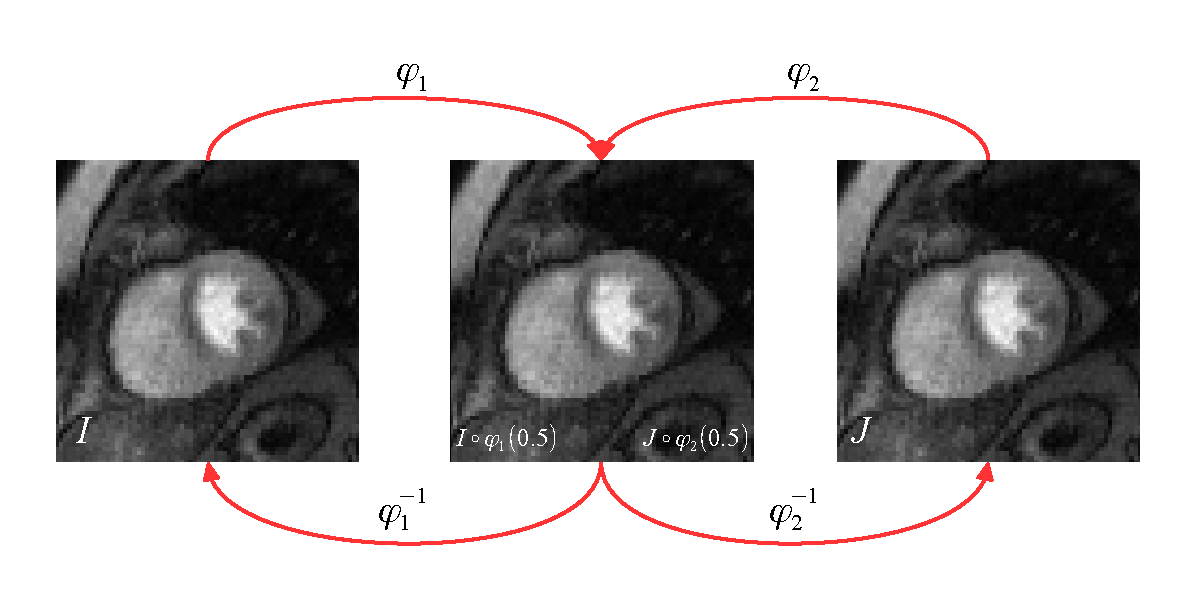
\includegraphics[width=0.9\linewidth]{../Figures/SyN.pdf}
\end{center}
Images $I$ and $J$ are registered by finding the optimal 
two transform pairs $\left(\phi_1,\phi_1^{-1}\right)$
  $\left(\phi_2,\phi_2^{-1}\right)$ which map to/from
  the respective images to the midway point. 
  Regularization using a fast B-spline fitting algorithm
  provides a contrast to the traditional Gaussian smoothing and has demonstrated
  measurable improvement in brain MR image normalization \cite{tustison2013}.

\vspace{0.5em} 
{\bf Transform composition to reference frame}
\vspace{0.5em} 
  
SyN yields both the forward and inverse transforms between images $I$ and $J$ denoted
as $I \underset{b}{\leftrightsquigarrow} J$ (where `$b$' denotes ``B-spline SyN'').
Thus, to transform any image, $I_t$, at time point, $t$, to the 
reference image, $I_R$, temporally located at time, $t=r$, we simply concatenate 
the transforms either forwards
\begin{align}
I_R  \underset{b_r}{\leftrightsquigarrow} \underset{b_{r+1}}{\leftrightsquigarrow} \cdots
      \underset{b_{t-2}}{\leftrightsquigarrow}\underset{b_{t-1}}{\leftrightsquigarrow} I_t
\end{align}
or backwards
\begin{align}
I_R  \underset{b_{r-1}}{\leftrightsquigarrow} \underset{b_{r-2}}{\leftrightsquigarrow} \cdots
      \underset{b_{t+1}}{\leftrightsquigarrow}\underset{b_t}{\leftrightsquigarrow} I_t.
\end{align}
By concatenating transforms, only a single interpolation is performed for each normalization 
to the reference frame.  

\vspace{0.3em}
}

%%%%%%%%%%%%%%%%%%%%%%%%%%%%%%%%%%%%%%%%%%%%%%%%%%%%%%%%%%%%%%%%%%%%%%%%%%%%%%
  \headerbox{ANTs Code}{name=code,column=1,span=1,below=bsyn,above=bottom}{
%%%%%%%%%%%%%%%%%%%%%%%%%%%%%%%%%%%%%%%%%%%%%%%%%%%%%%%%%%%%%%%%%%%%%%%%%%%%%%

\begin{lstlisting}^^J
# Input image pairs include:^^J
#  \ \ * N4 bias corrected^^J
#  \ \ * Structure-preserving noise reduction (SUSAN) of N4 images^^J
#  \ \ * Laplacian filtering of SUSAN images.^^J
^^J
antsRegistration --dimensionality 2 \\^^J
\ \ \ \ \ \ \ \ \ \ \ \ \ \ \ \ \ --output $\{outputPrefix\} \\^^J
\ \ \ \ \ \ \ \ \ \ \ \ \ \ \ \ \ --winsorize-image-intensities [0.01,0.99] \\^^J
\ \ \ \ \ \ \ \ \ \ \ \ \ \ \ \ \ --use-histogram-matching 1 \\^^J
\ \ \ \ \ \ \ \ \ \ \ \ \ \ \ \ \ --transform BSplineSyN[0.1,2x2,0] \\^^J
\ \ \ \ \ \ \ \ \ \ \ \ \ \ \ \ \ --metric CC[$\{n4Fxd\},$\{n4Mvng\},1,6] \\^^J
\ \ \ \ \ \ \ \ \ \ \ \ \ \ \ \ \ --metric Demons[$\{susanFxd\},$\{susanMvng\},1,1] \\^^J
\ \ \ \ \ \ \ \ \ \ \ \ \ \ \ \ \ --metric Demons[$\{laplacianFxd\},$\{laplacianMvng\},1,1] \\^^J
\ \ \ \ \ \ \ \ \ \ \ \ \ \ \ \ \ --convergence [100x70x50,1e-8,10] \\^^J
\ \ \ \ \ \ \ \ \ \ \ \ \ \ \ \ \ --shrink-factors 4x2x1 \\^^J
\ \ \ \ \ \ \ \ \ \ \ \ \ \ \ \ \ --smoothing-sigmas 1x0.5x0vox^^J
\end{lstlisting}

  }


%%%%%%%%%%%%%%%%%%%%%%%%%%%%%%%%%%%%%%%%%%%%%%%%%%%%%%%%%%%%%%%%%%%%%%%%%%%%%%
  \headerbox{Evaluation}{name=evaluation,column=2,span=1}{
%%%%%%%%%%%%%%%%%%%%%%%%%%%%%%%%%%%%%%%%%%%%%%%%%%%%%%%%%%%%%%%%%%%%%%%%%%%%%%
\vspace{0.3em}

{\bf Tissue and arterial input function time plots}
\vspace{-0.3em}

\begin{center}
 \makebox[\linewidth][c]{
   \begin{tabular}{ccccc}
    {} & \multicolumn{2}{c}{\tiny \bf Rest} &  \multicolumn{2}{c}{\tiny \bf Stress} \\
    \rotatebox{90}{\tiny \bf\,\,\,\,\,\,\,MoCo\_01} & 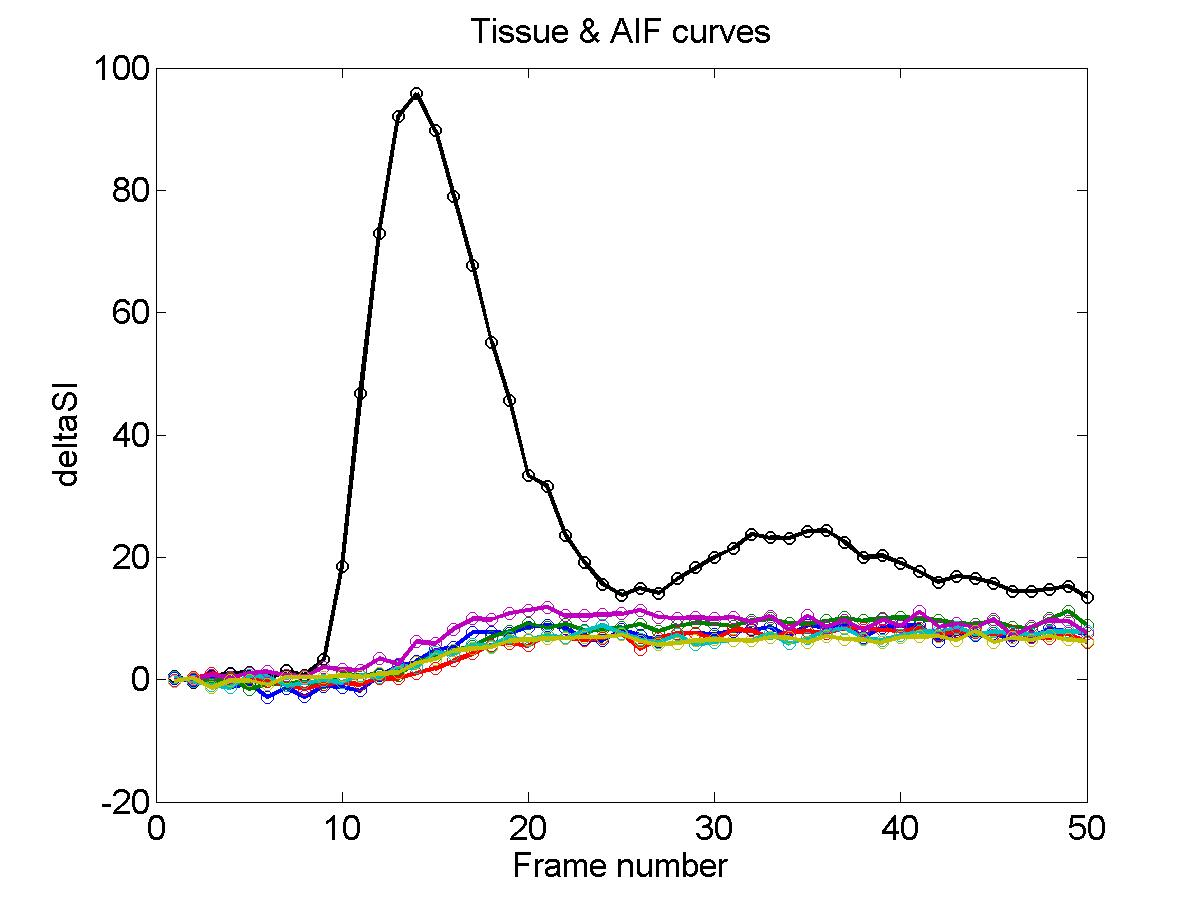
\includegraphics[width=17mm]{../Figures/Results_jpg_DZnomask/MoCo_01_DZNoMask_Rest_Curve.jpg} 
    \hspace{-5mm} &
    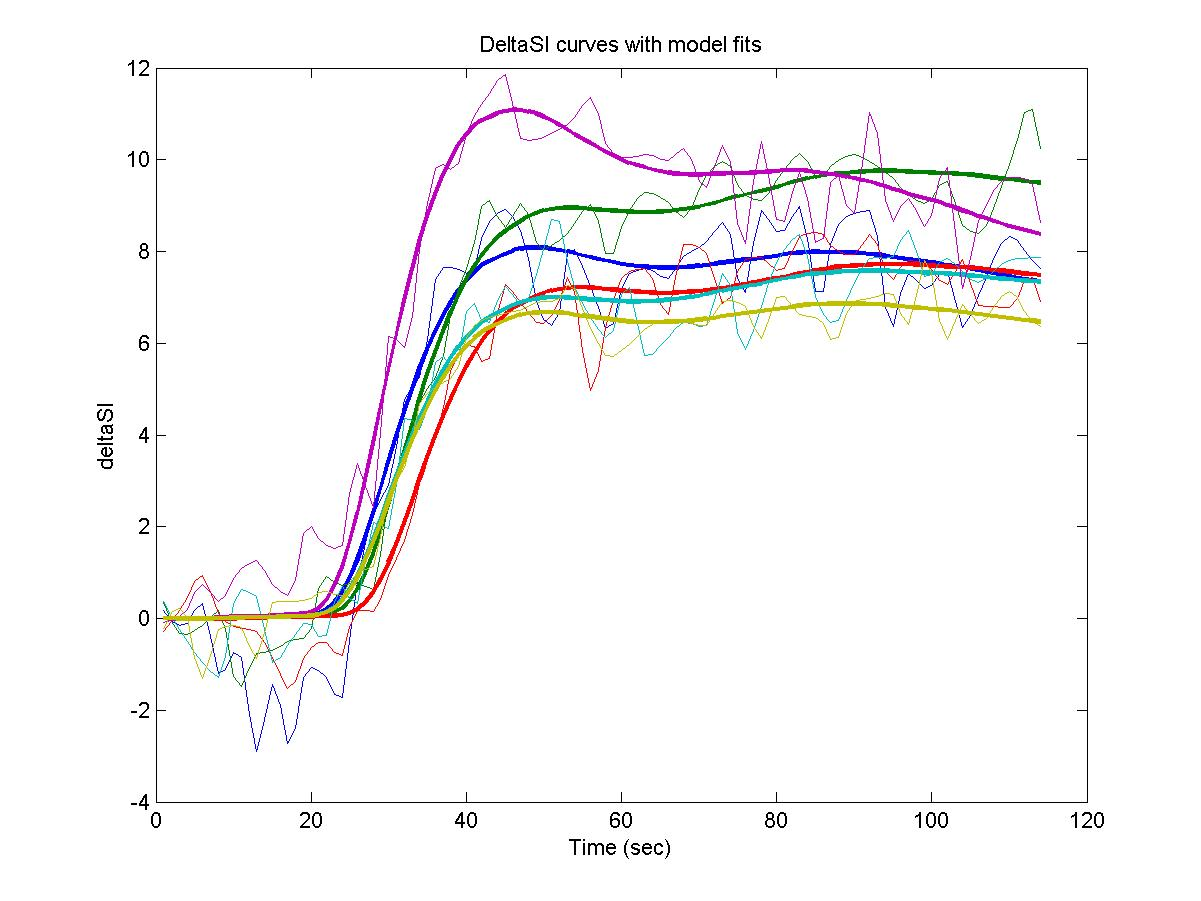
\includegraphics[width=17mm]{../Figures/Results_jpg_DZnomask/MoCo_01_DZNoMask_Rest_Fit.jpg} 
    \hspace{-5mm} &
    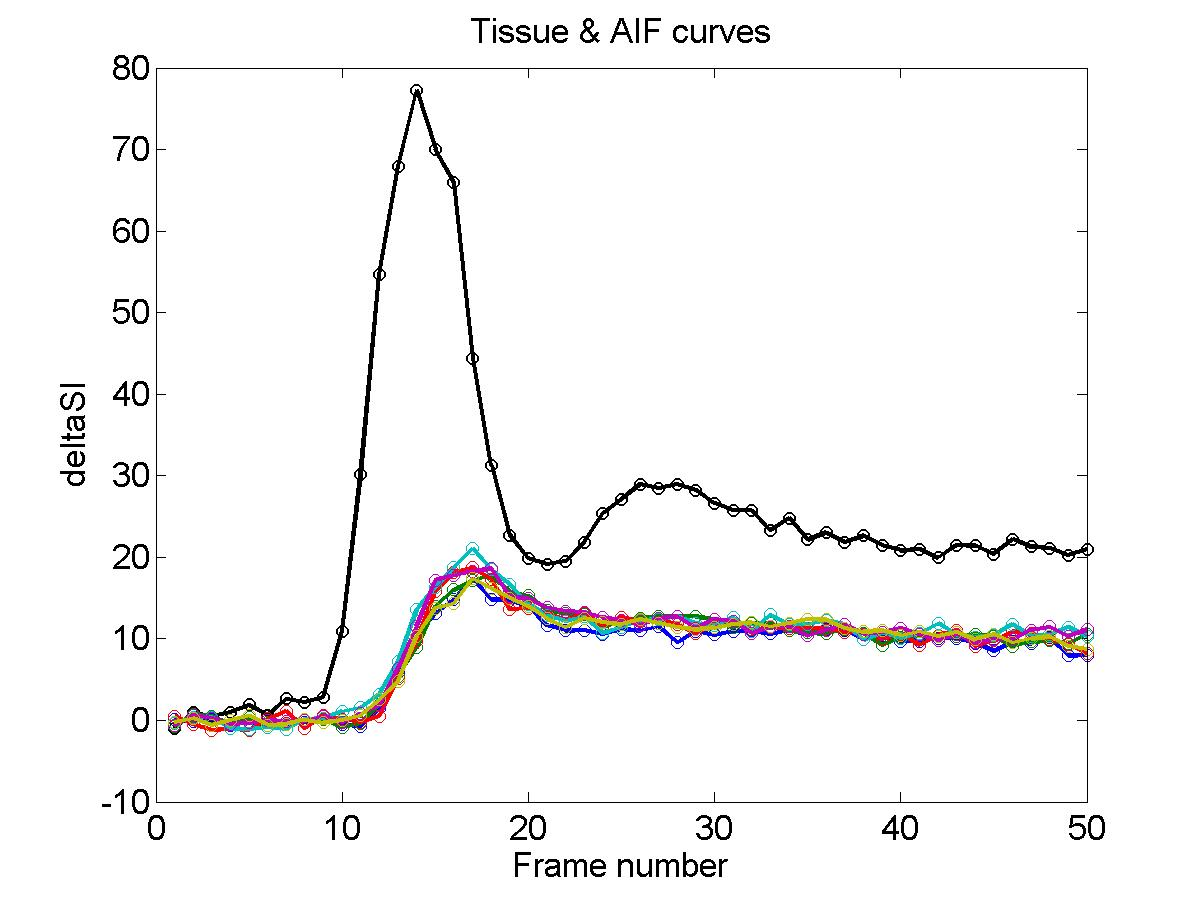
\includegraphics[width=17mm]{../Figures/Results_jpg_DZnomask/MoCo_01_DZNoMask_Stress_Curve.jpg} 
    \hspace{-5mm} &
    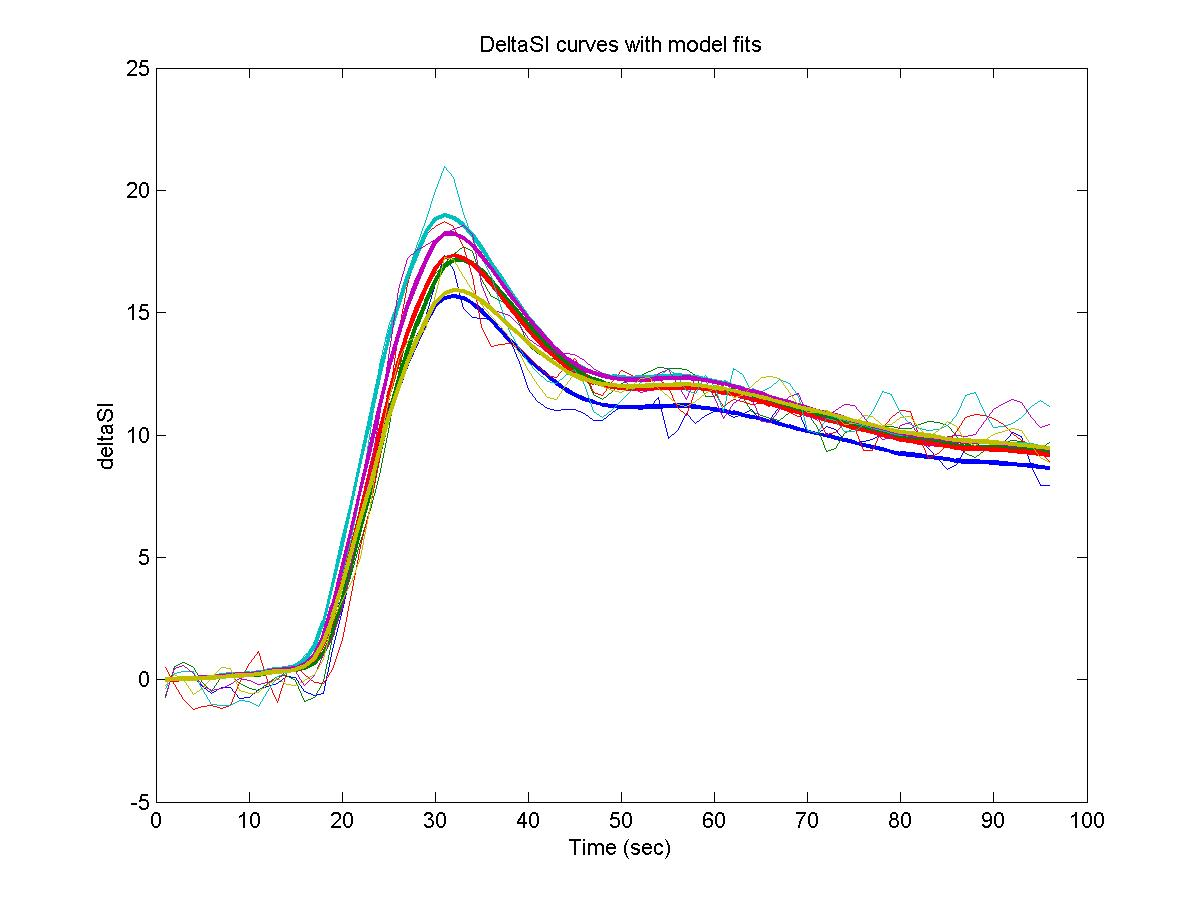
\includegraphics[width=17mm]{../Figures/Results_jpg_DZnomask/MoCo_01_DZNoMask_Stress_Fit.jpg} \\
    \rotatebox{90}{\tiny \bf\,\,\,\,\,\,\,MoCo\_02} & 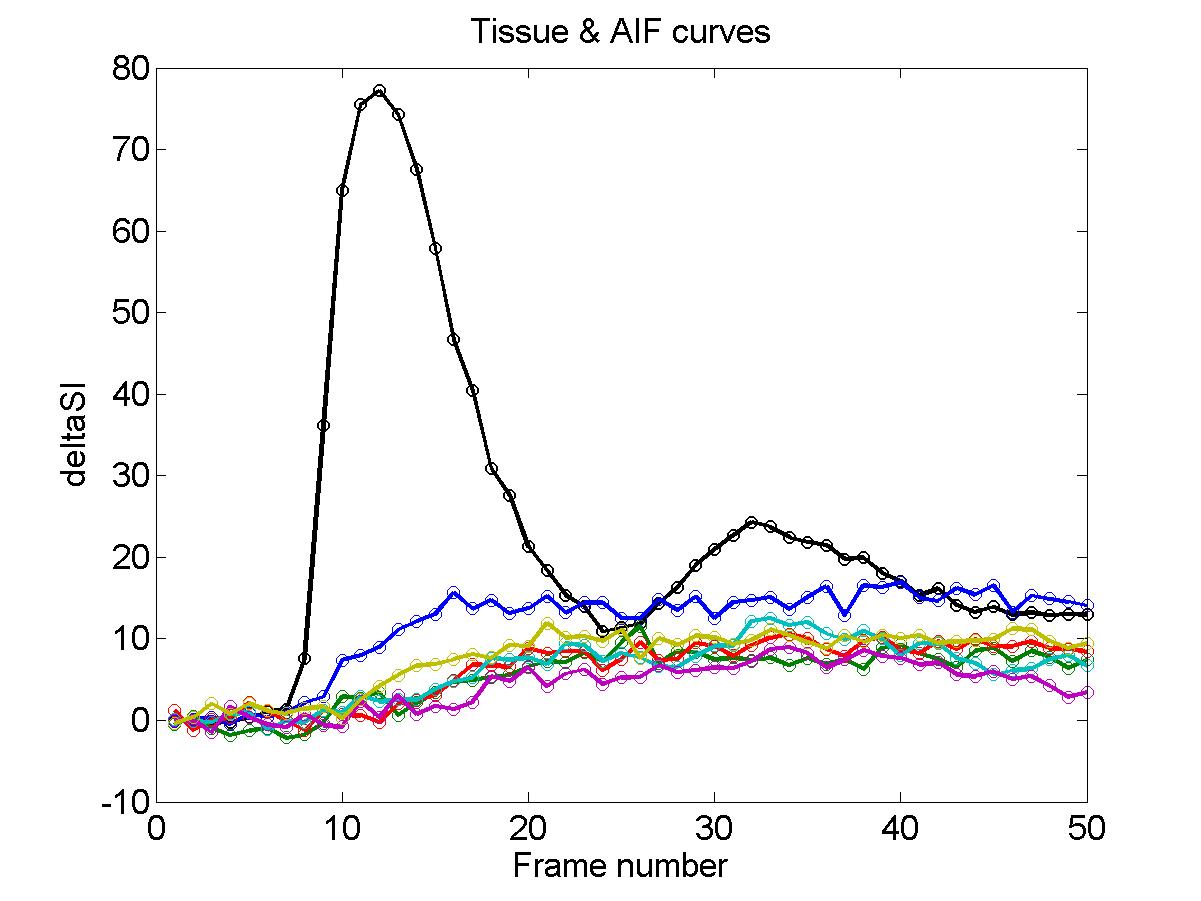
\includegraphics[width=17mm]{../Figures/Results_jpg_DZnomask/MoCo_02_DZNoMask_Rest_Curve.jpg} 
    \hspace{-5mm} &
    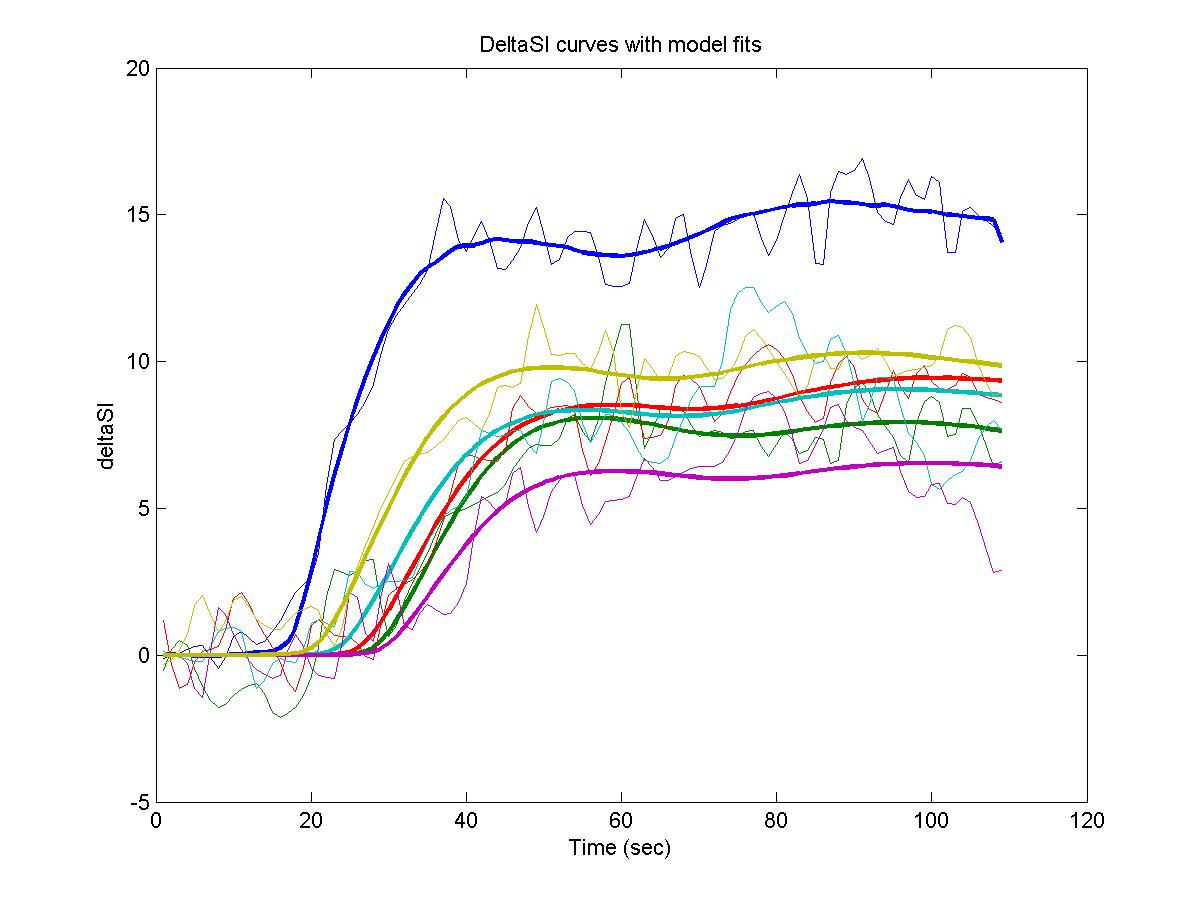
\includegraphics[width=17mm]{../Figures/Results_jpg_DZnomask/MoCo_02_DZNoMask_Rest_Fit.jpg} 
    \hspace{-5mm} &
    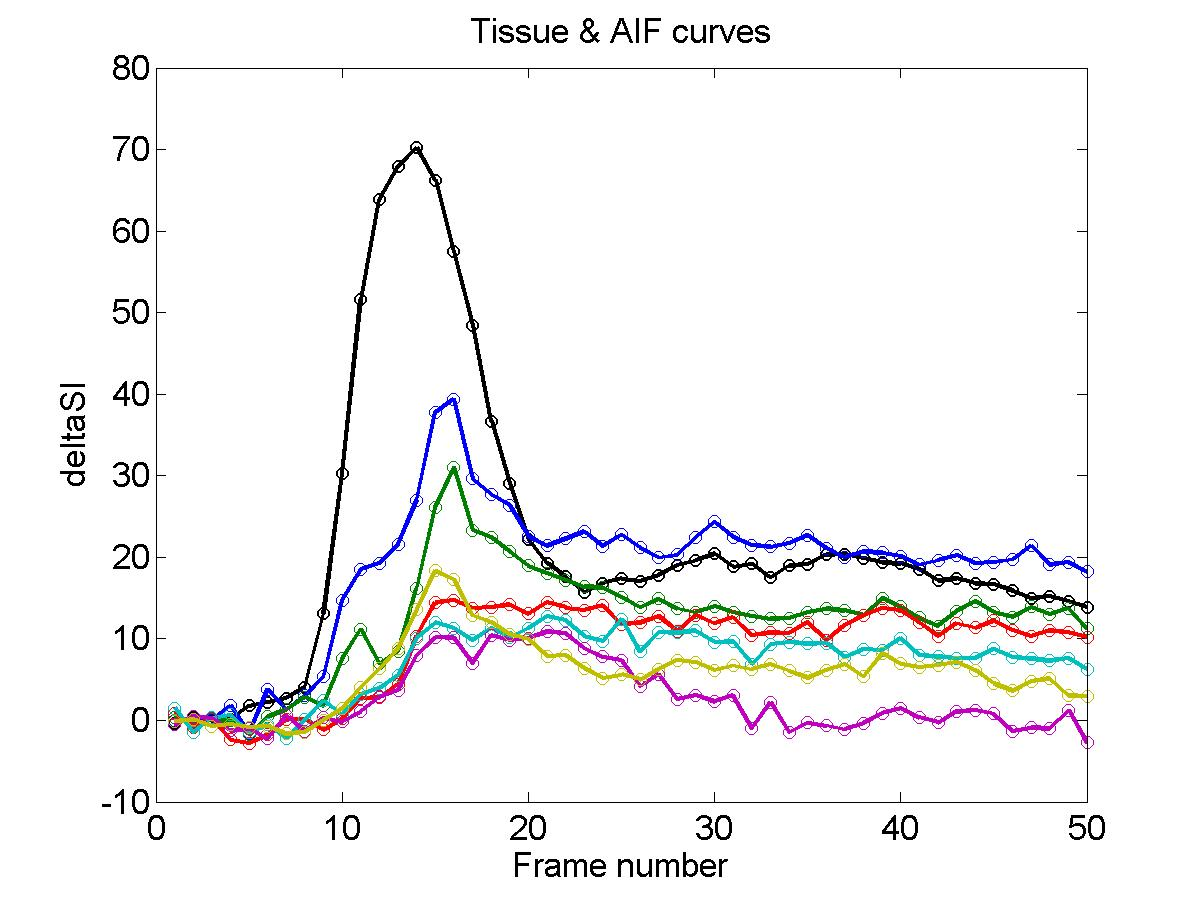
\includegraphics[width=17mm]{../Figures/Results_jpg_DZnomask/MoCo_02_DZNoMask_Stress_Curve.jpg} 
    \hspace{-5mm} &
    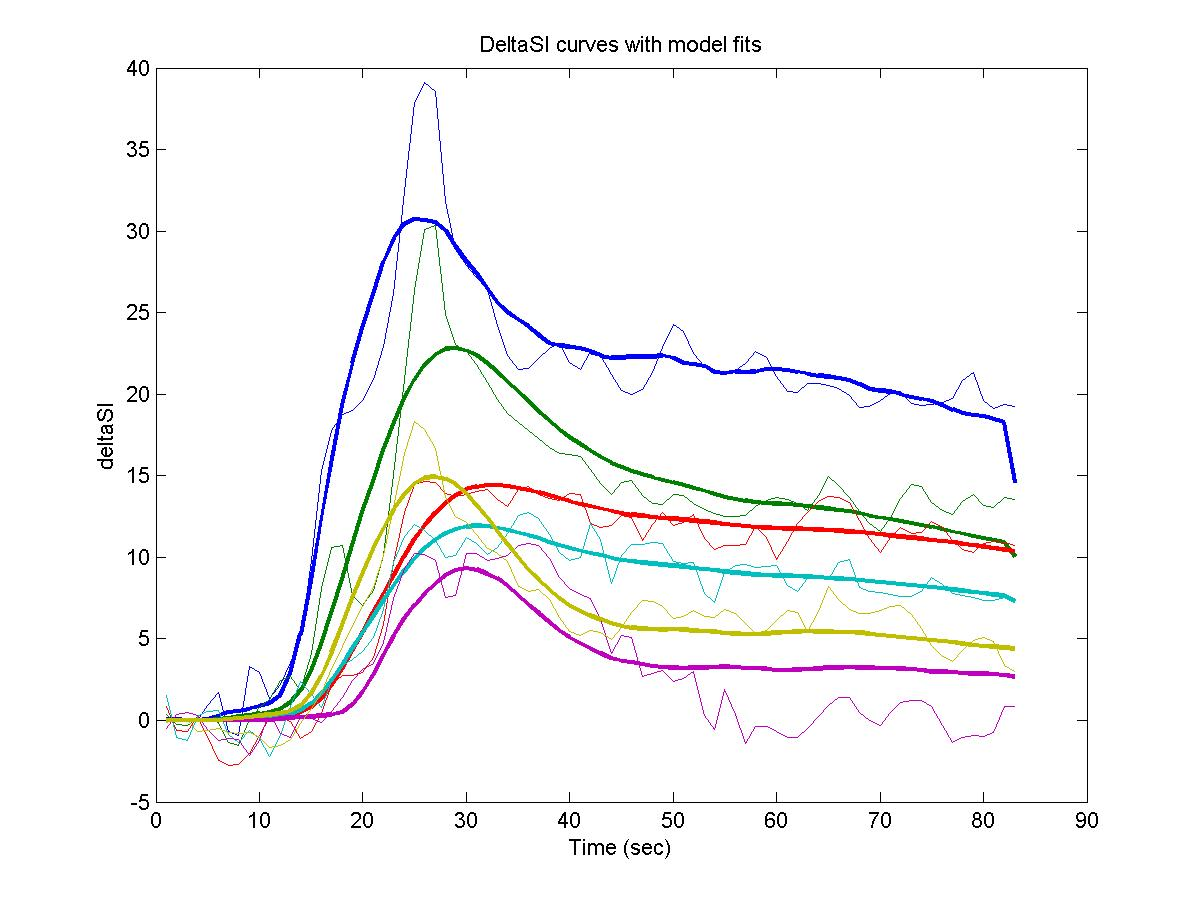
\includegraphics[width=17mm]{../Figures/Results_jpg_DZnomask/MoCo_02_DZNoMask_Stress_Fit.jpg} \\
    \rotatebox{90}{\tiny \bf\,\,\,\,\,\,\,MoCo\_03} & 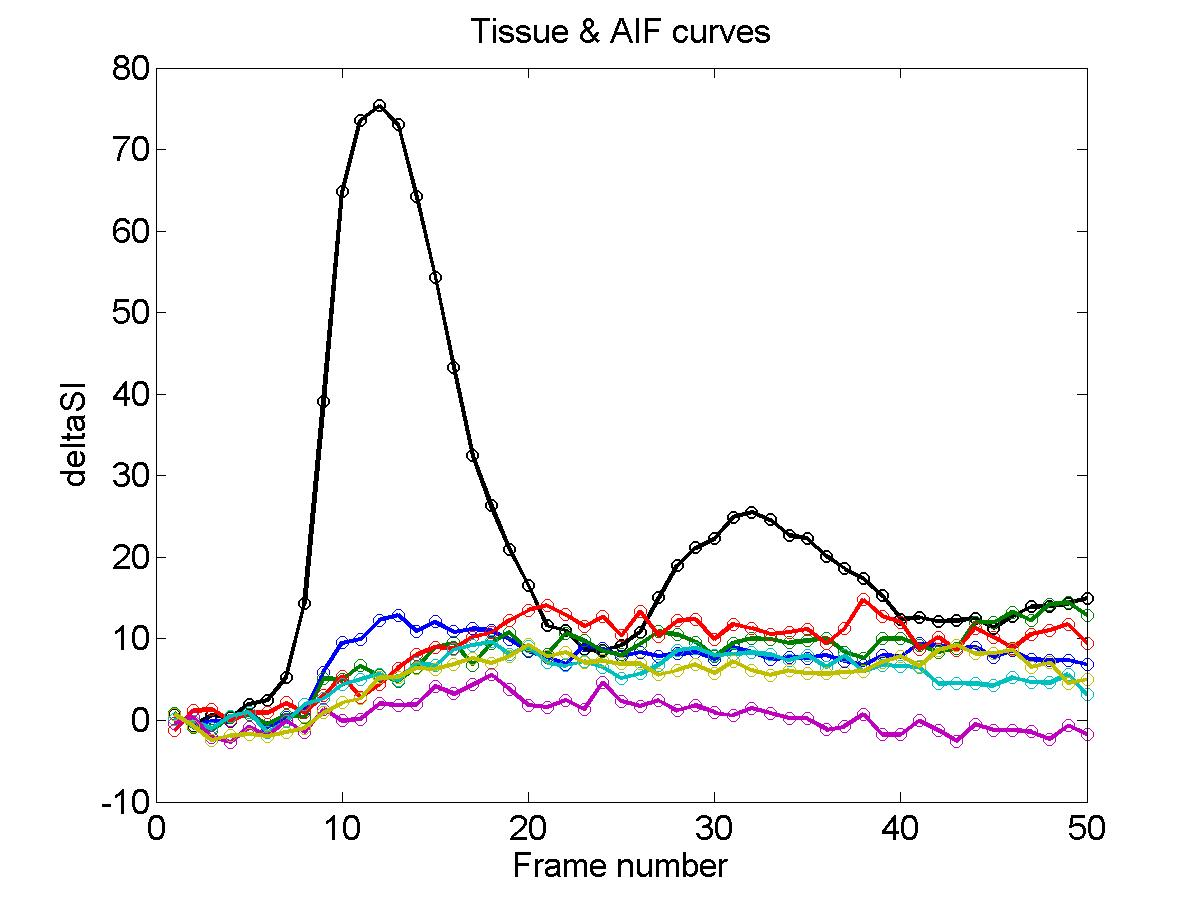
\includegraphics[width=17mm]{../Figures/Results_jpg_DZnomask/MoCo_03_DZNoMask_Rest_Curve.jpg} 
    \hspace{-5mm} &
    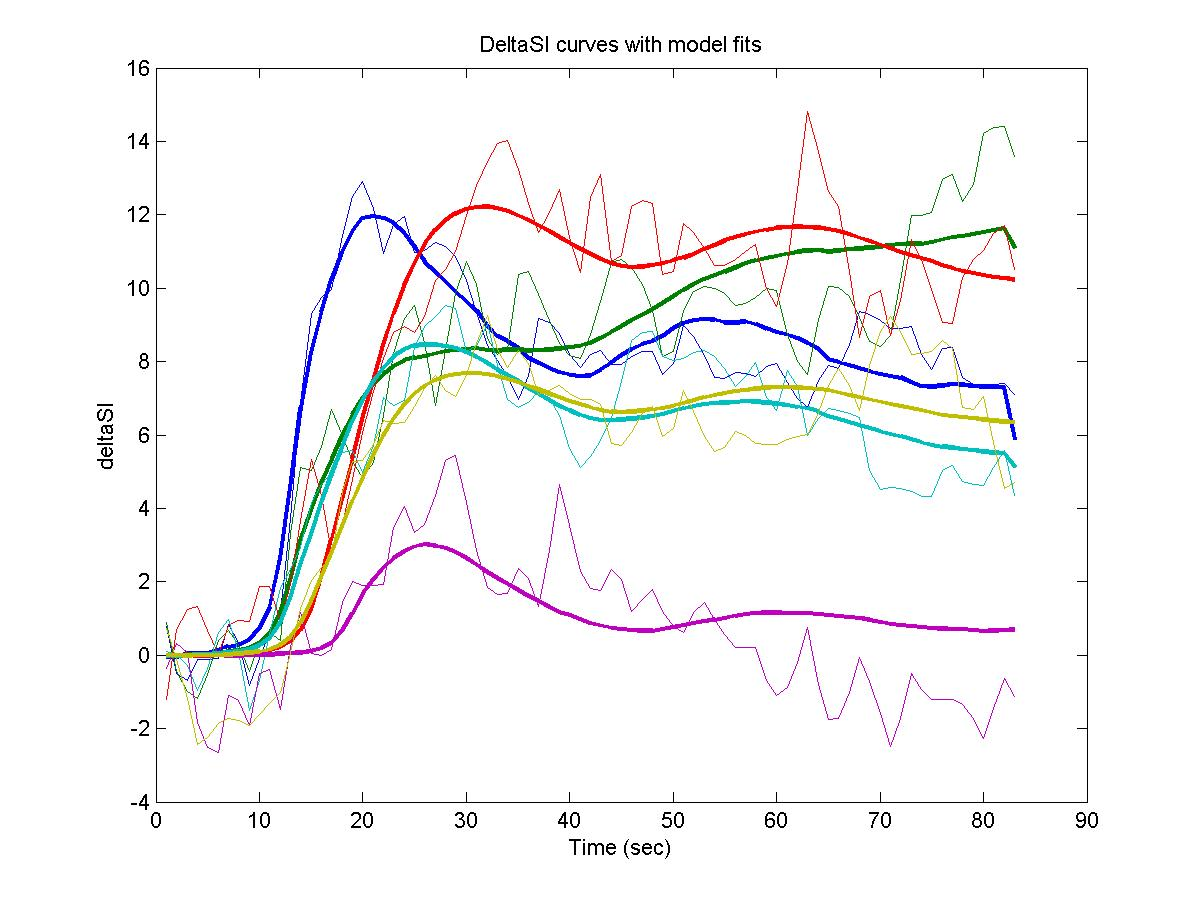
\includegraphics[width=17mm]{../Figures/Results_jpg_DZnomask/MoCo_03_DZNoMask_Rest_Fit.jpg} 
    \hspace{-5mm} &
    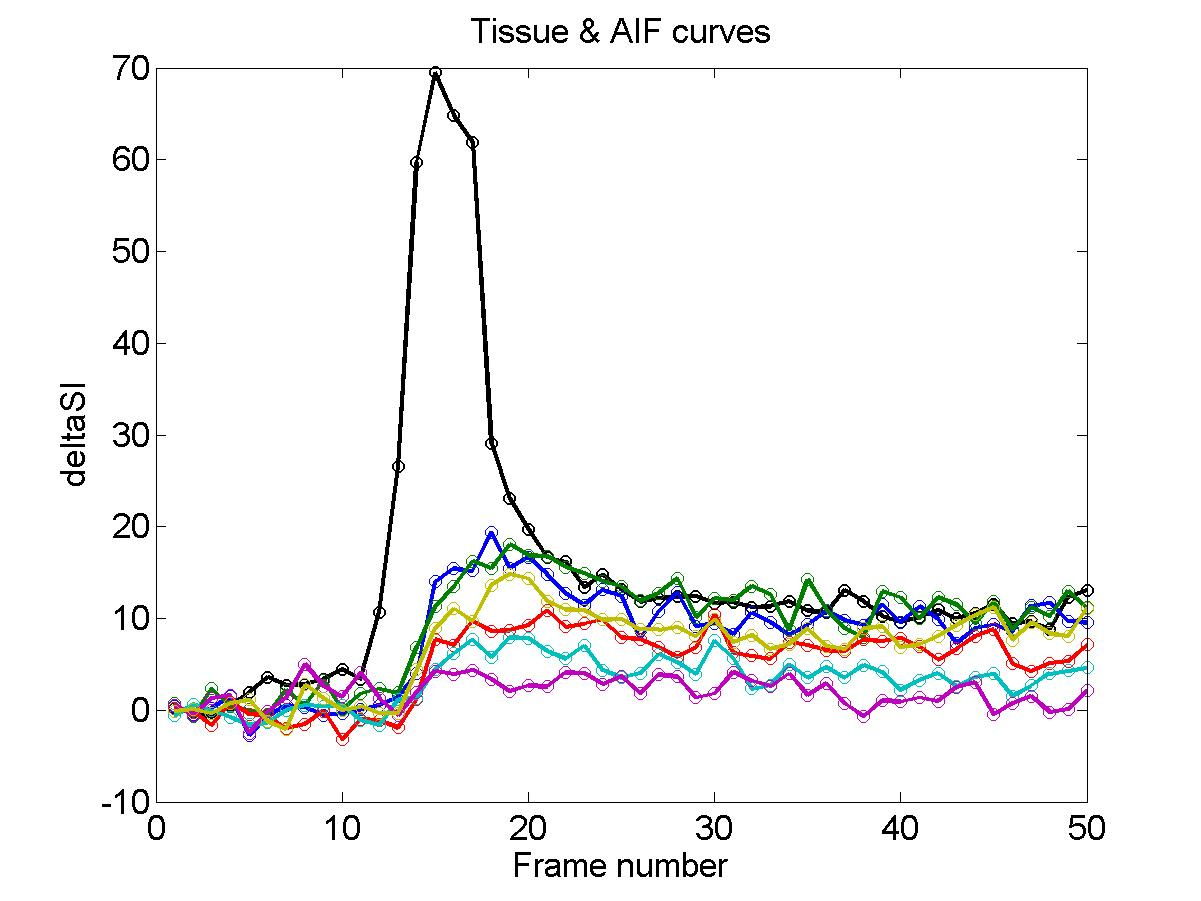
\includegraphics[width=17mm]{../Figures/Results_jpg_DZnomask/MoCo_03_DZNoMask_Stress_Curve.jpg} 
    \hspace{-5mm} &
    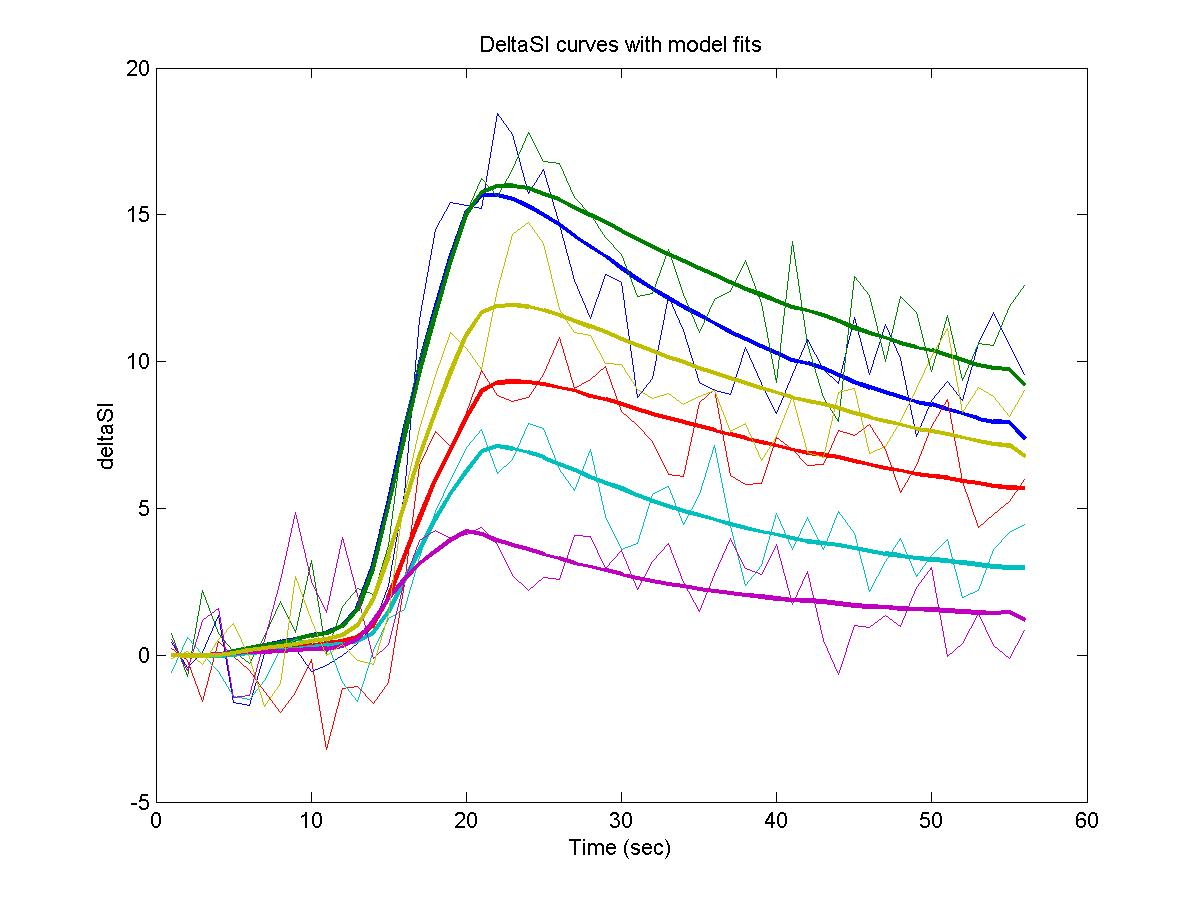
\includegraphics[width=17mm]{../Figures/Results_jpg_DZnomask/MoCo_03_DZNoMask_Stress_Fit.jpg} \\
    \rotatebox{90}{\tiny \bf\,\,\,\,\,\,\,MoCo\_04} & 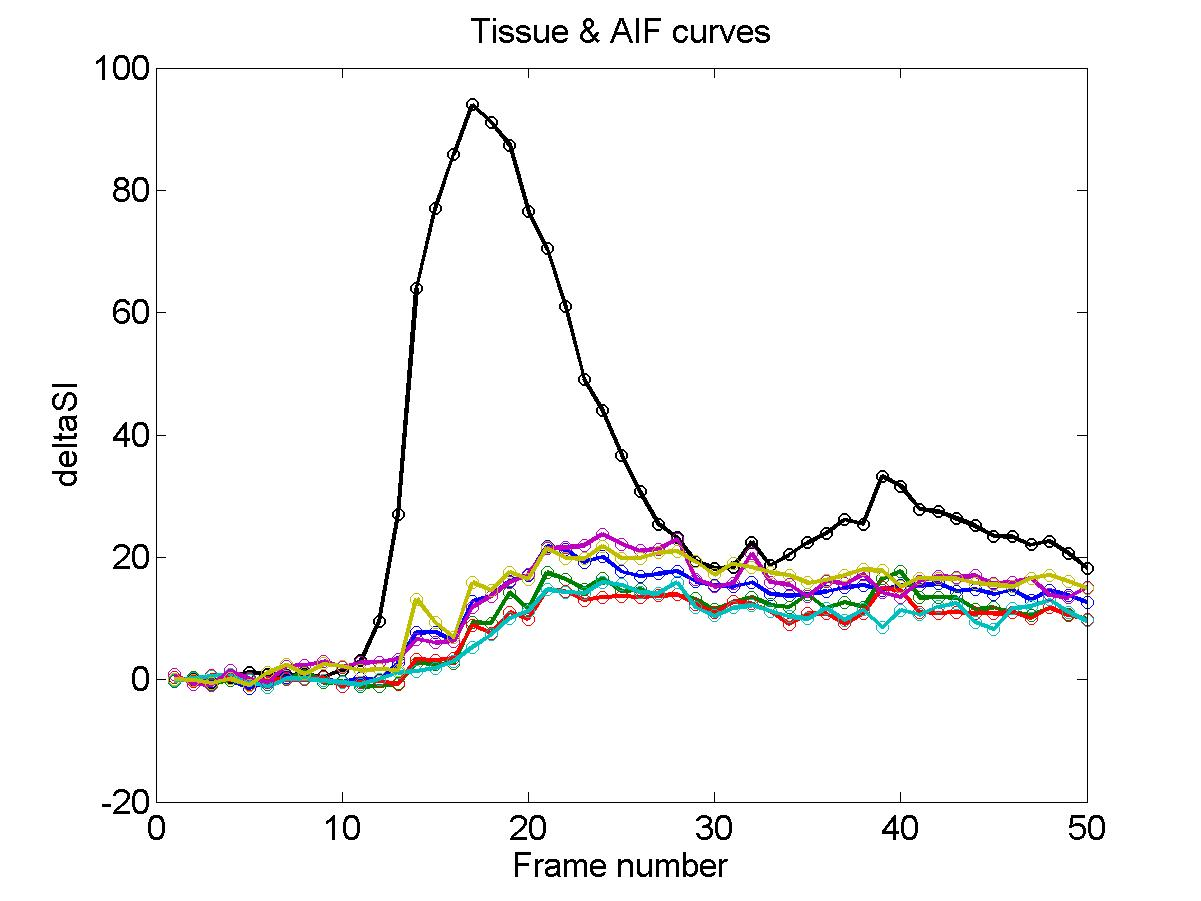
\includegraphics[width=17mm]{../Figures/Results_jpg_DZnomask/MoCo_04_DZNoMask_Rest_Curve.jpg} 
    \hspace{-5mm} &
    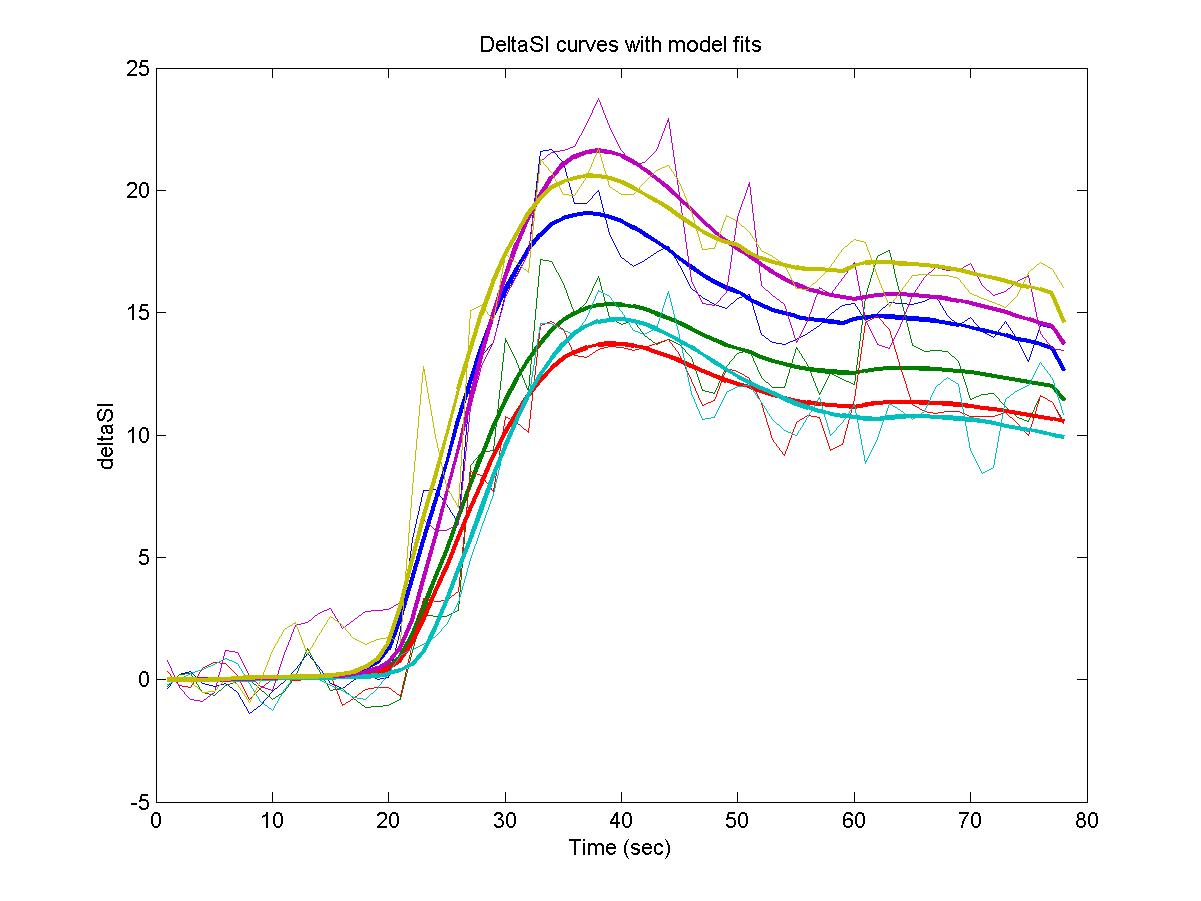
\includegraphics[width=17mm]{../Figures/Results_jpg_DZnomask/MoCo_04_DZNoMask_Rest_Fit.jpg} 
    \hspace{-5mm} &
    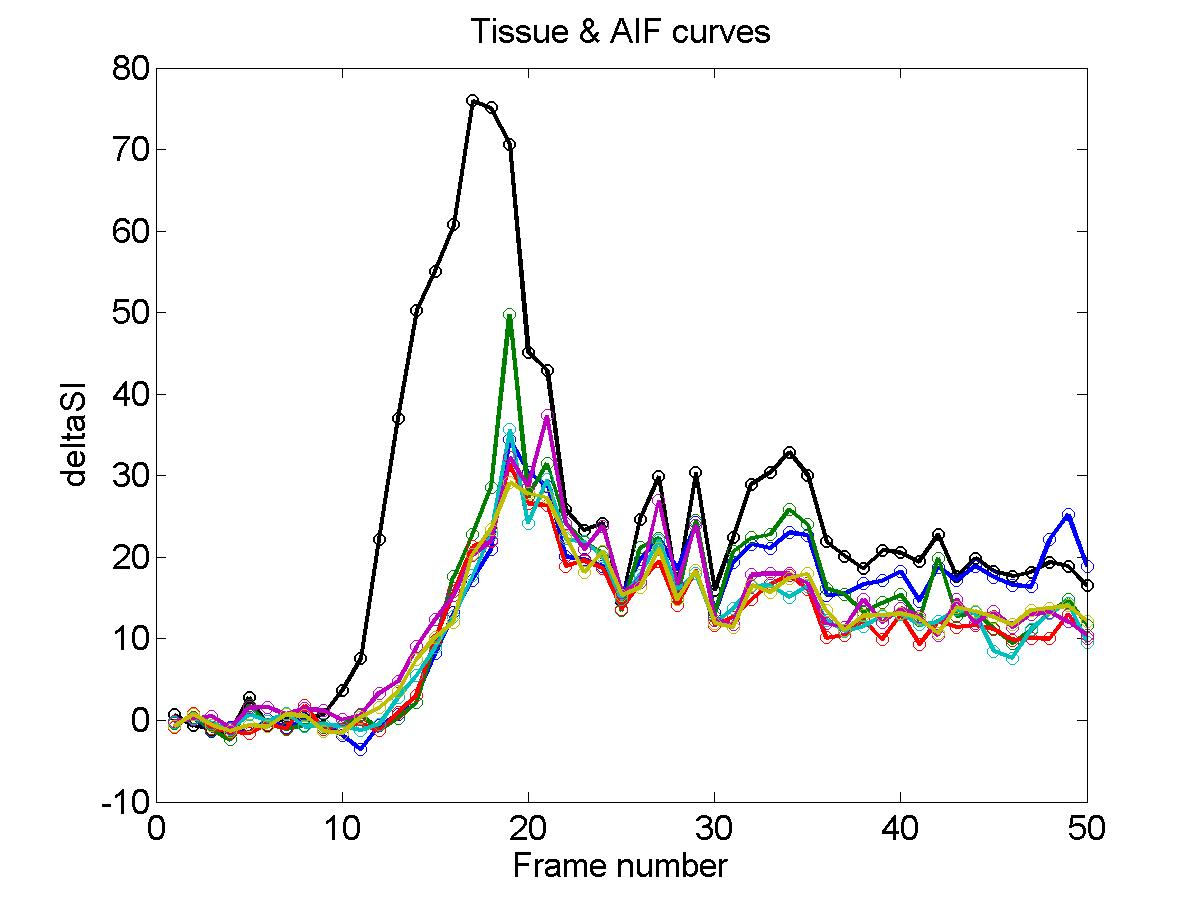
\includegraphics[width=17mm]{../Figures/Results_jpg_DZnomask/MoCo_04_DZNoMask_Stress_Curve.jpg} 
    \hspace{-5mm} &
    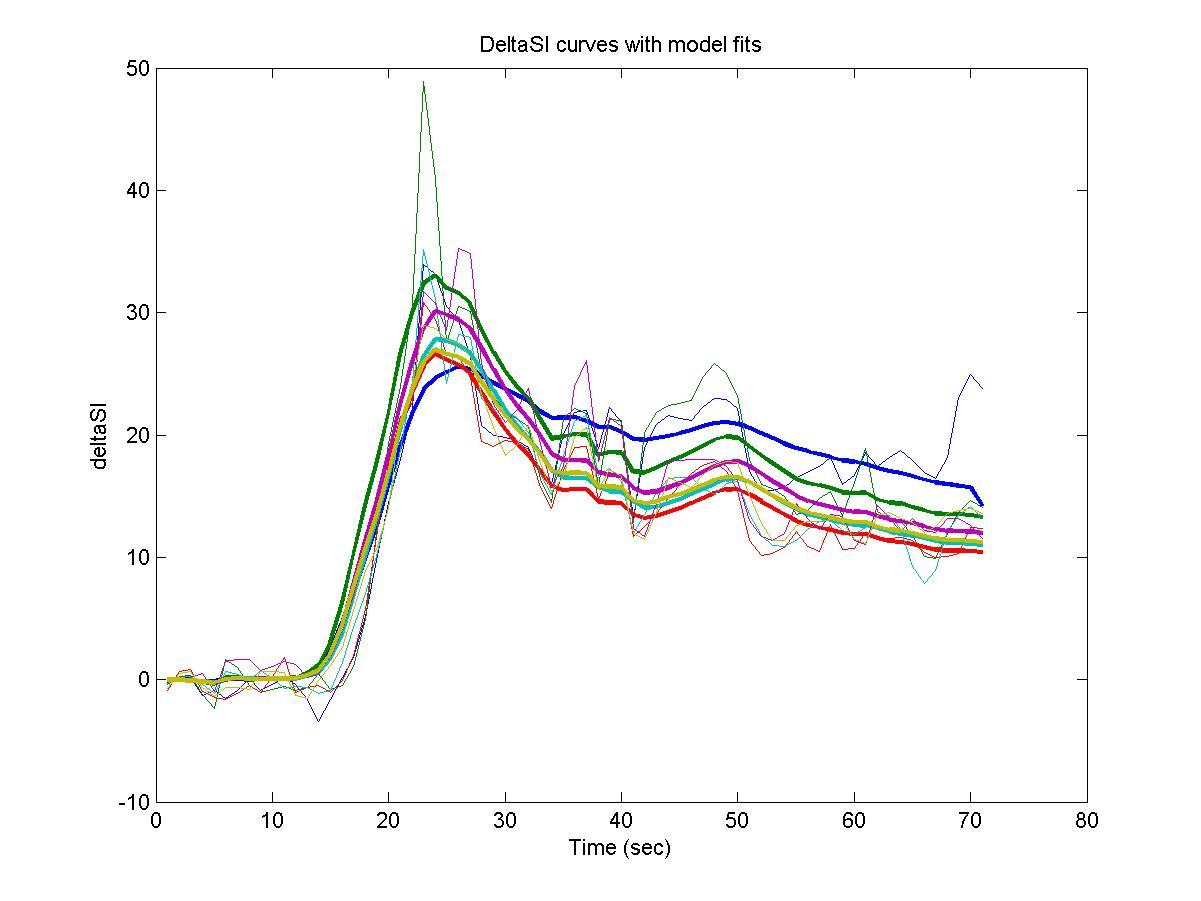
\includegraphics[width=17mm]{../Figures/Results_jpg_DZnomask/MoCo_04_DZNoMask_Stress_Fit.jpg} \\
    \rotatebox{90}{\tiny \bf\,\,\,\,\,\,\,MoCo\_05} & 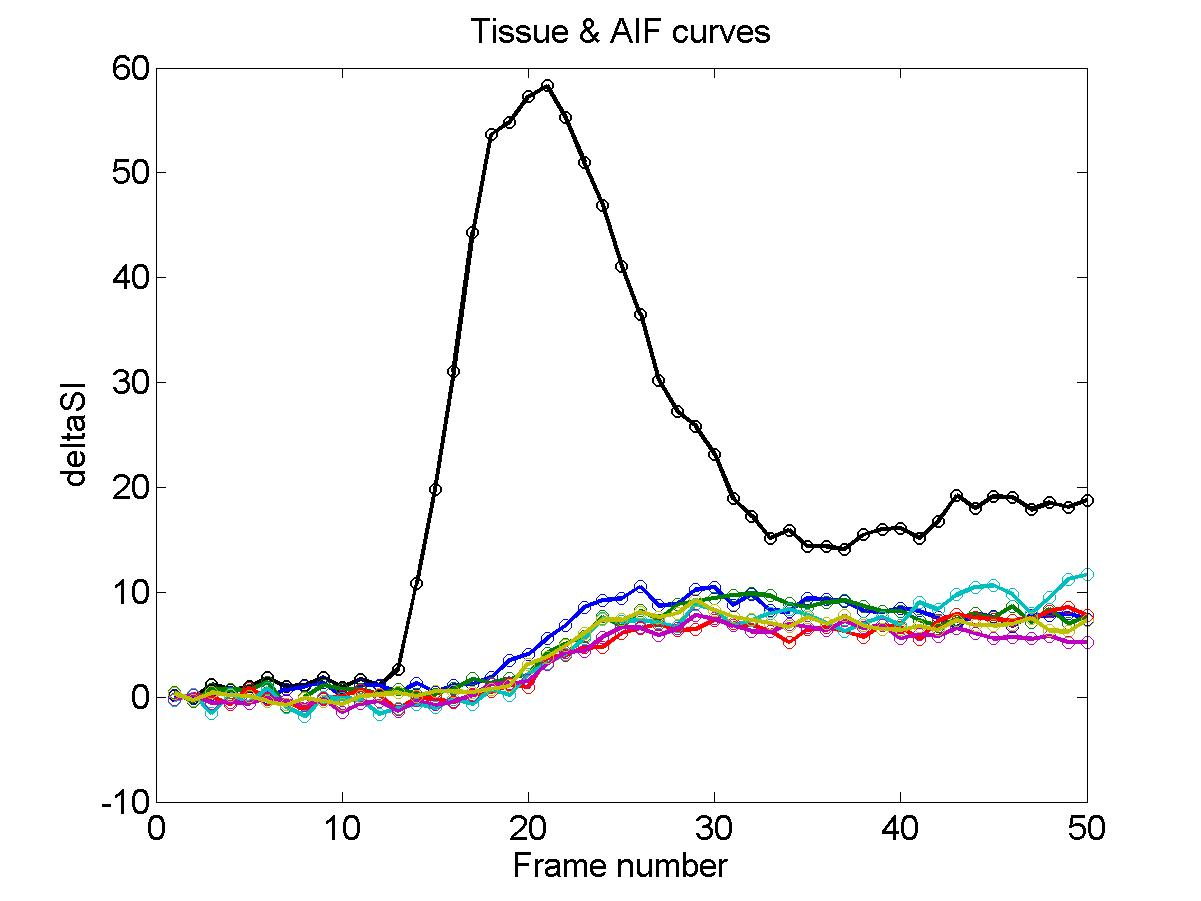
\includegraphics[width=17mm]{../Figures/Results_jpg_DZnomask/MoCo_05_DZNoMask_Rest_Curve.jpg} 
    \hspace{-5mm} &
    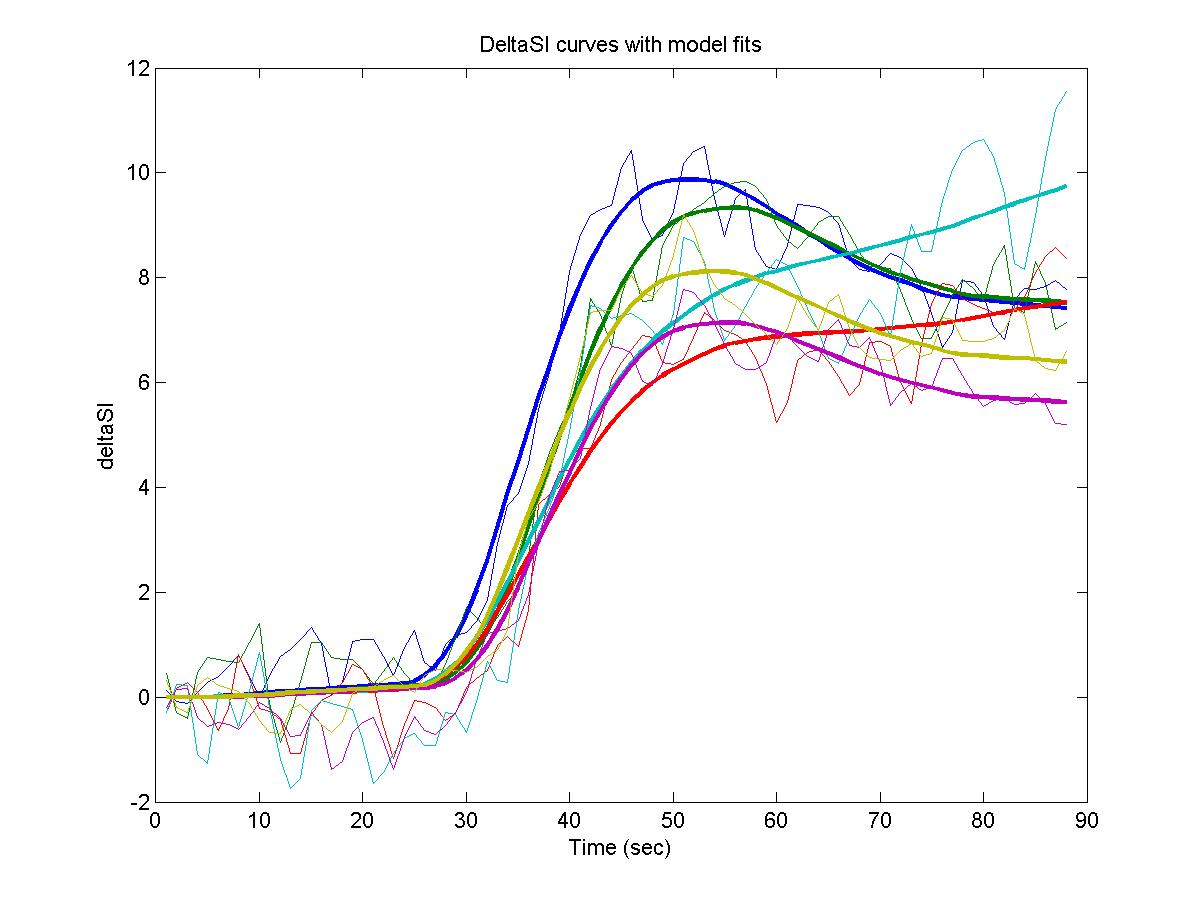
\includegraphics[width=17mm]{../Figures/Results_jpg_DZnomask/MoCo_05_DZNoMask_Rest_Fit.jpg} 
    \hspace{-5mm} &
    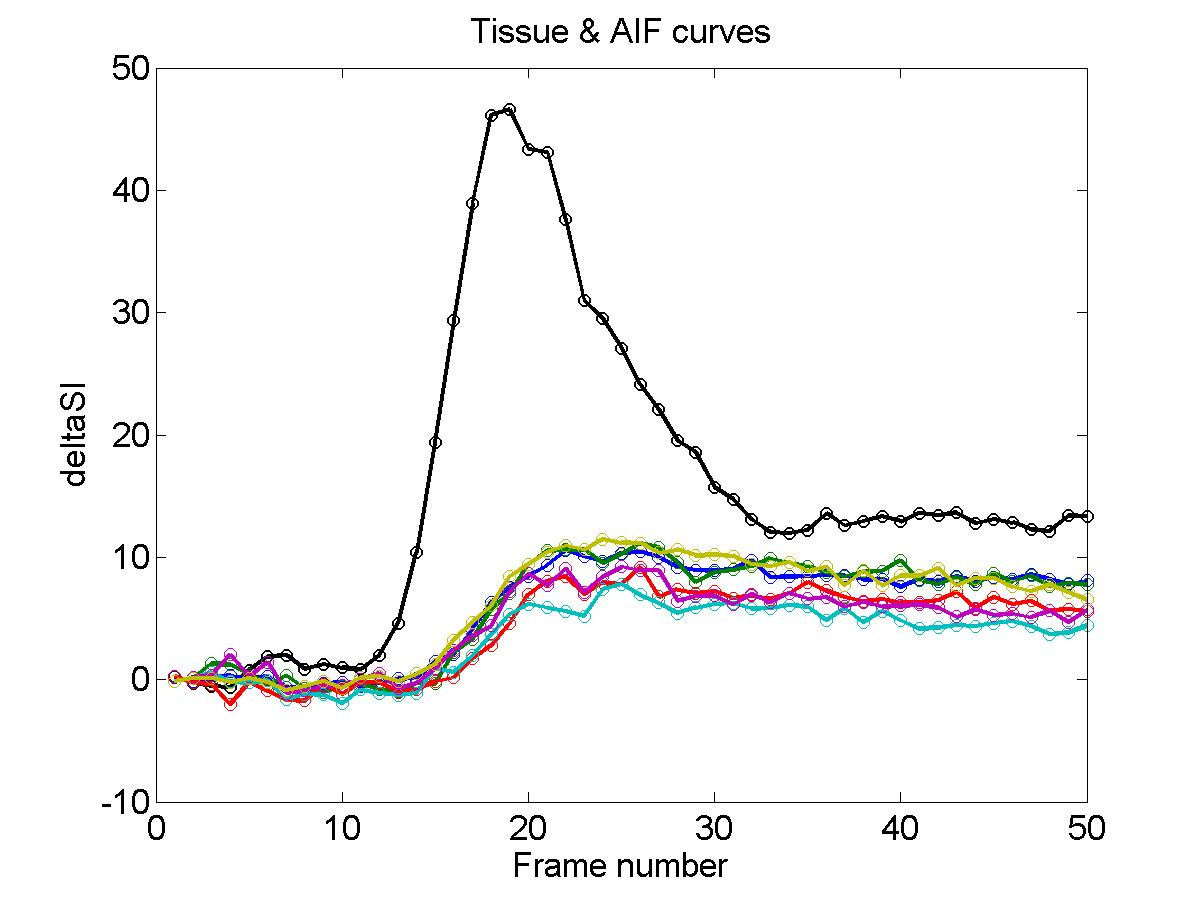
\includegraphics[width=17mm]{../Figures/Results_jpg_DZnomask/MoCo_05_DZNoMask_Stress_Curve.jpg} 
    \hspace{-5mm} &
    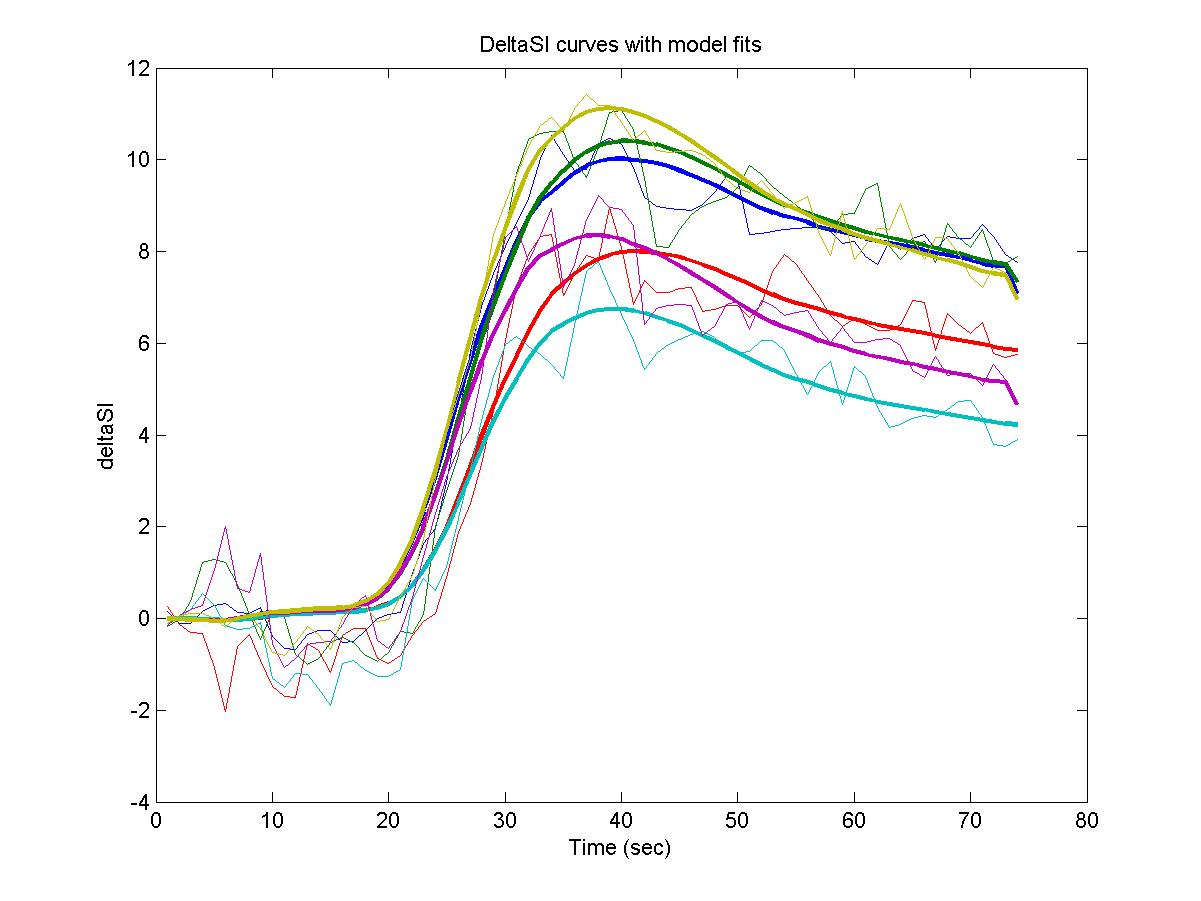
\includegraphics[width=17mm]{../Figures/Results_jpg_DZnomask/MoCo_05_DZNoMask_Stress_Fit.jpg} \\
    \rotatebox{90}{\tiny \bf\,\,\,\,\,\,\,MoCo\_06} & 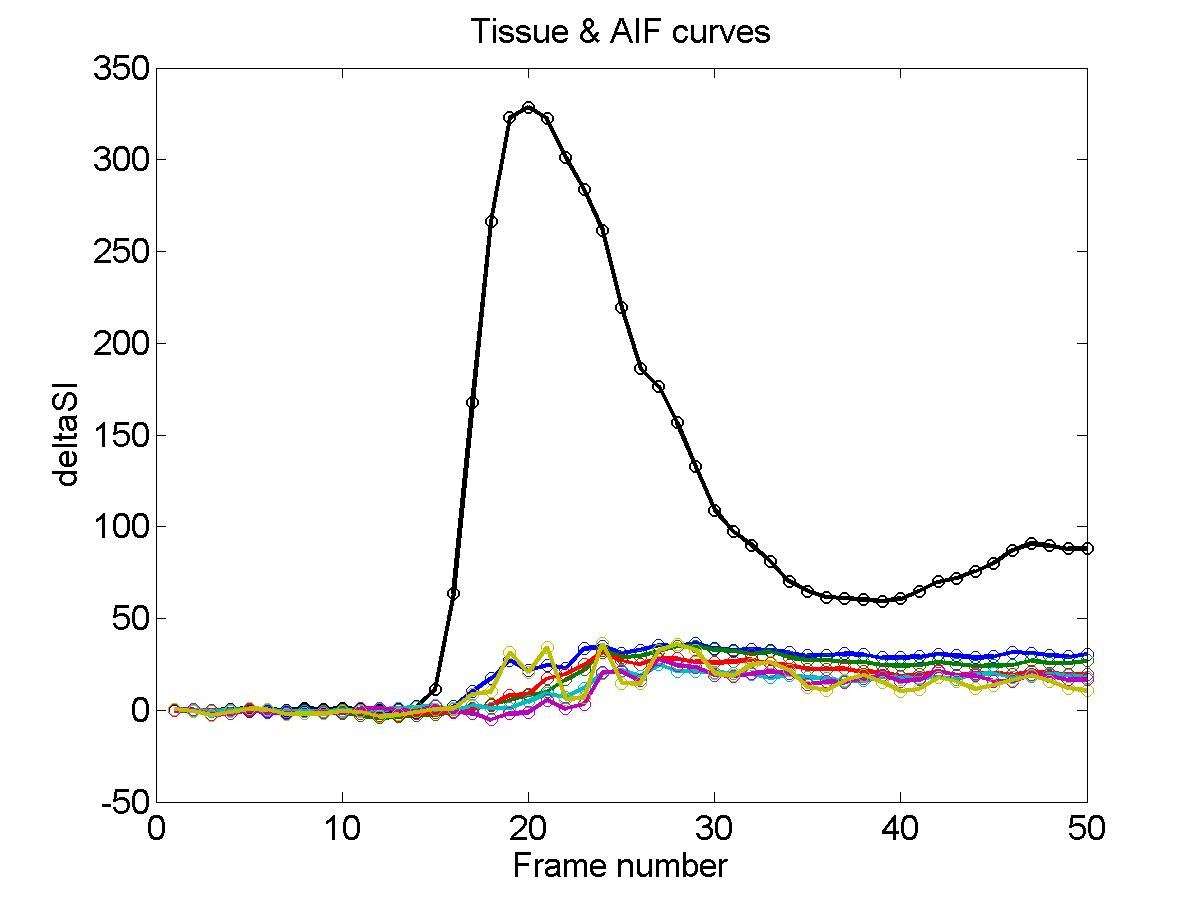
\includegraphics[width=17mm]{../Figures/Results_jpg_DZnomask/MoCo_06_DZNoMask_Rest_Curve.jpg} 
    \hspace{-5mm} &
    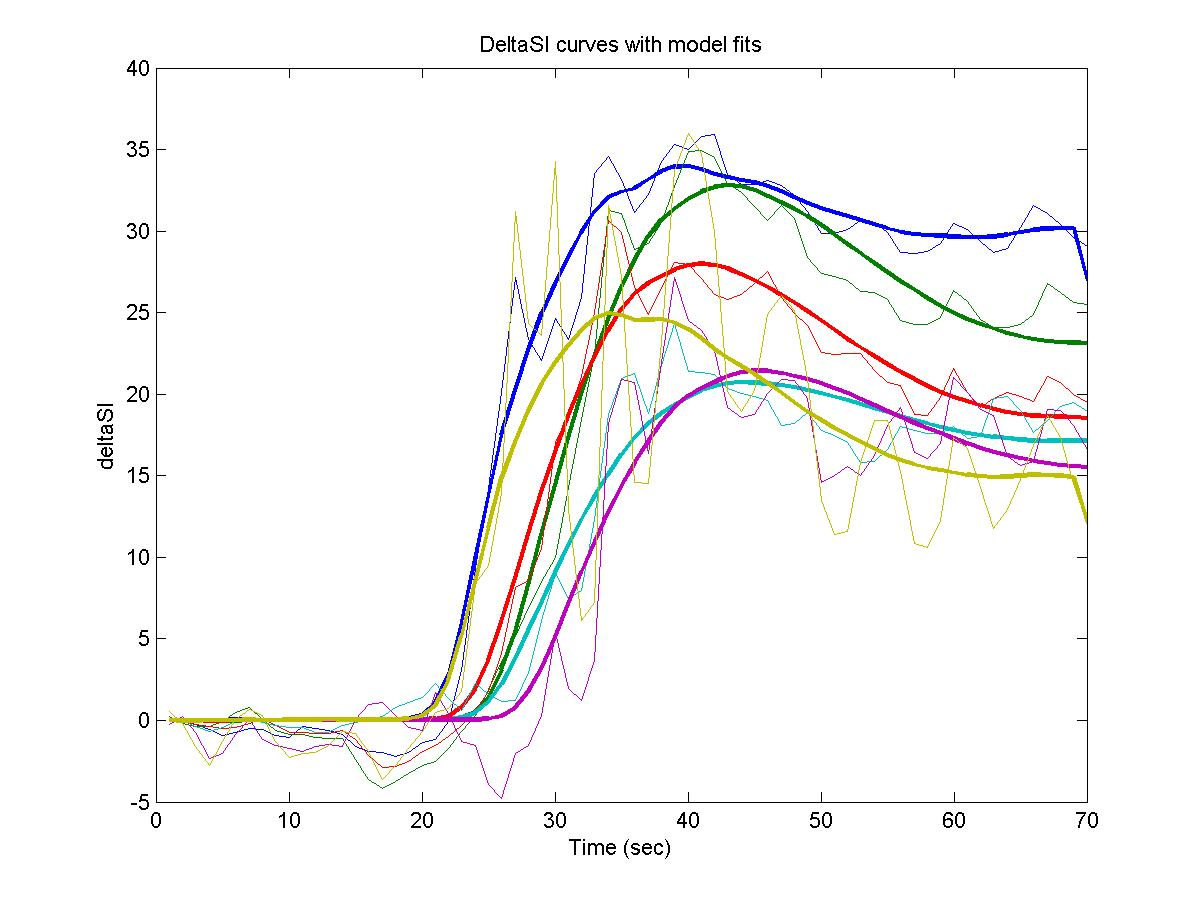
\includegraphics[width=17mm]{../Figures/Results_jpg_DZnomask/MoCo_06_DZNoMask_Rest_Fit.jpg} 
    \hspace{-5mm} &
    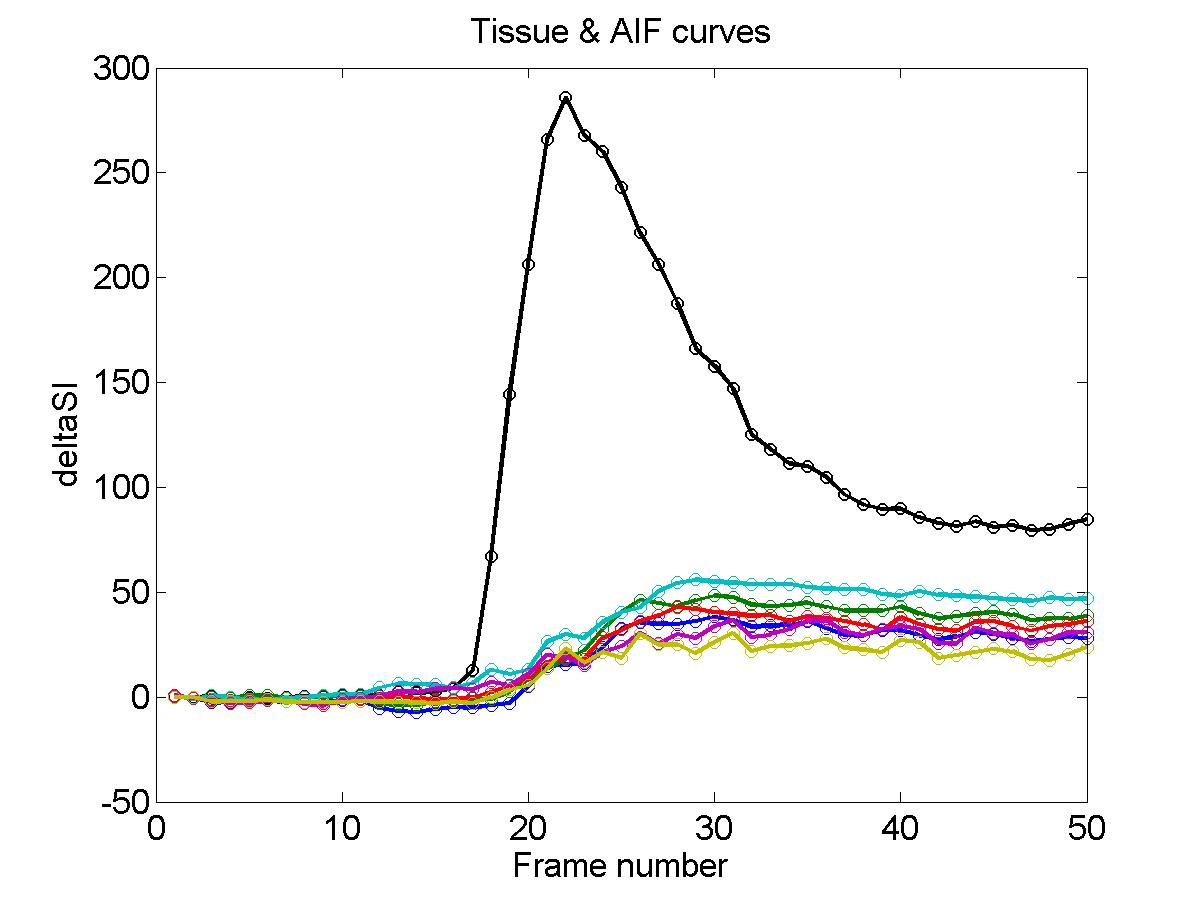
\includegraphics[width=17mm]{../Figures/Results_jpg_DZnomask/MoCo_06_DZNoMask_Stress_Curve.jpg} 
    \hspace{-5mm} &
    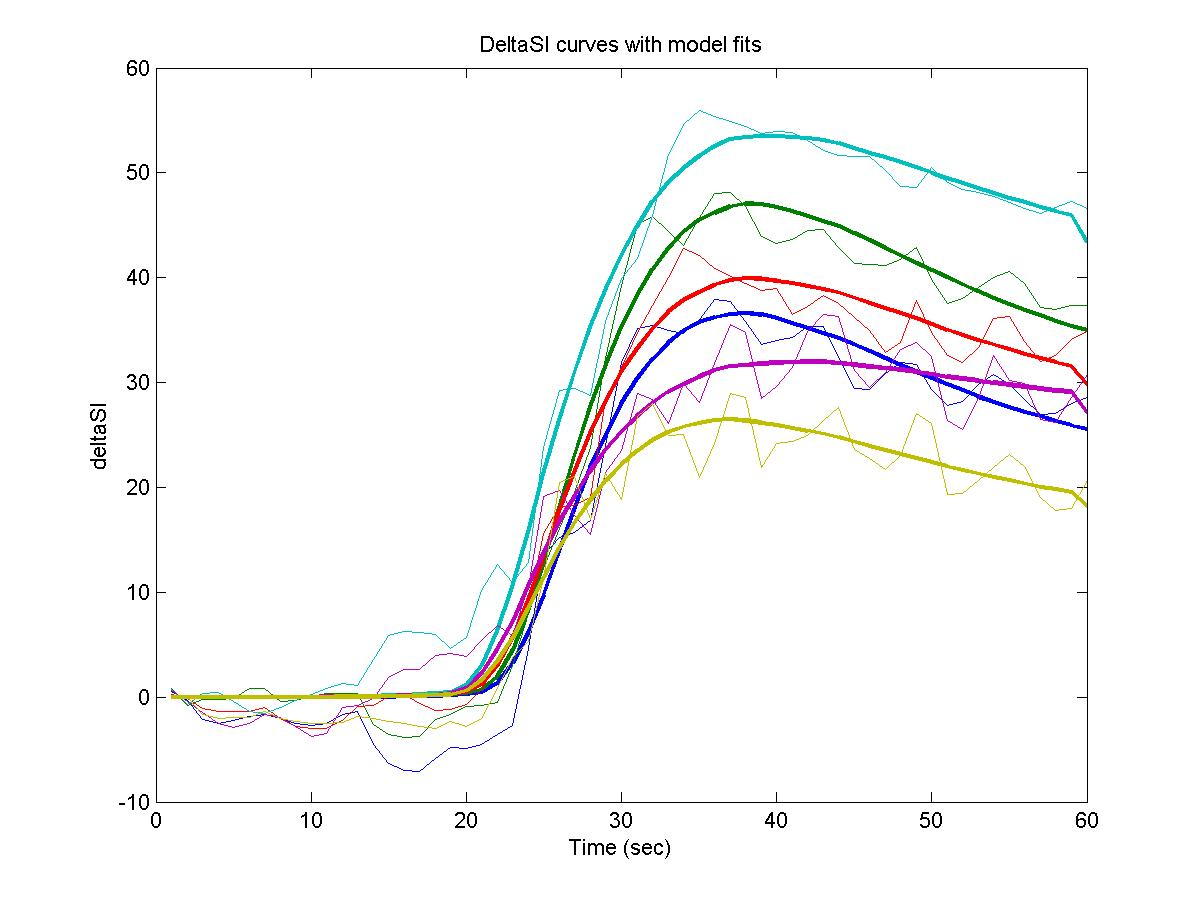
\includegraphics[width=17mm]{../Figures/Results_jpg_DZnomask/MoCo_06_DZNoMask_Stress_Fit.jpg} \\
    \rotatebox{90}{\tiny \bf\,\,\,\,\,\,\,MoCo\_07} & 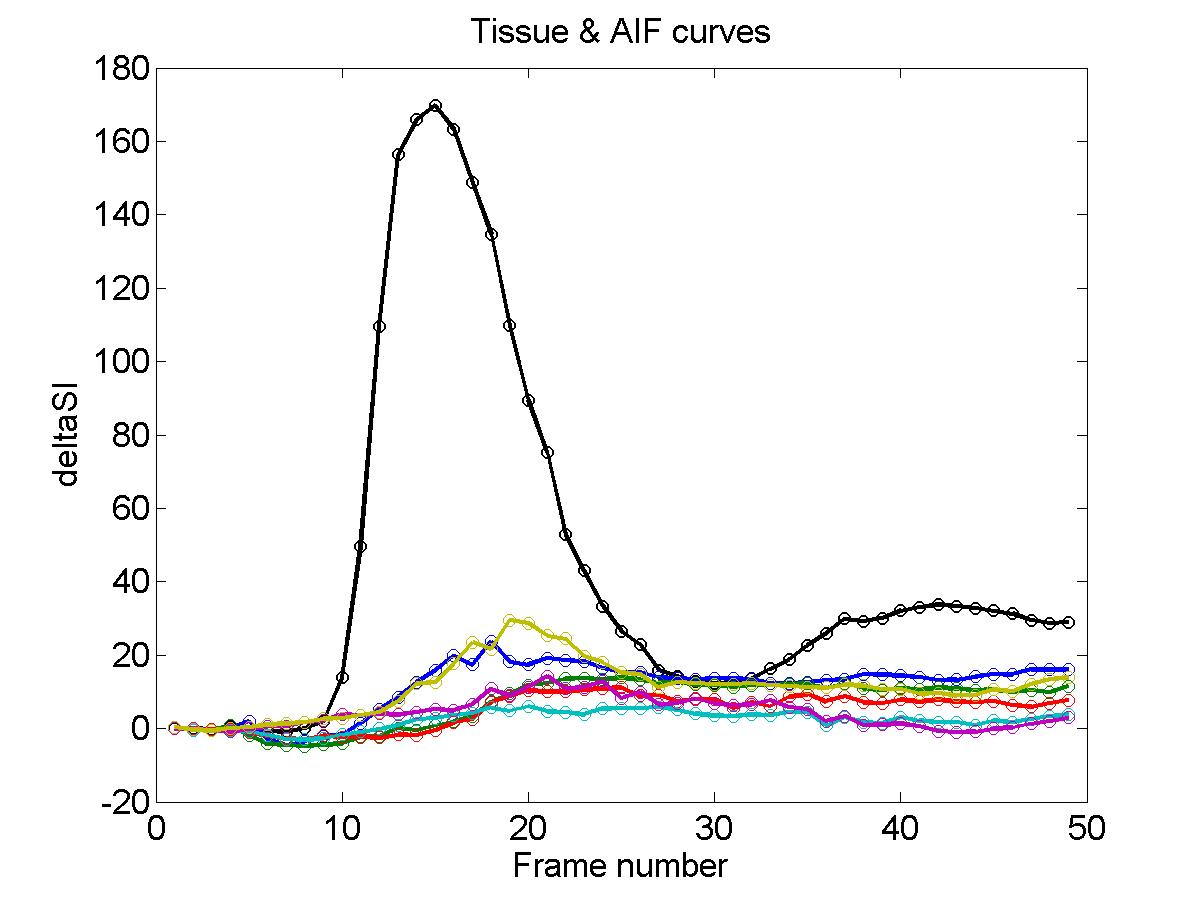
\includegraphics[width=17mm]{../Figures/Results_jpg_DZnomask/MoCo_07_DZNoMask_Rest_Curve.jpg} 
    \hspace{-5mm} &
    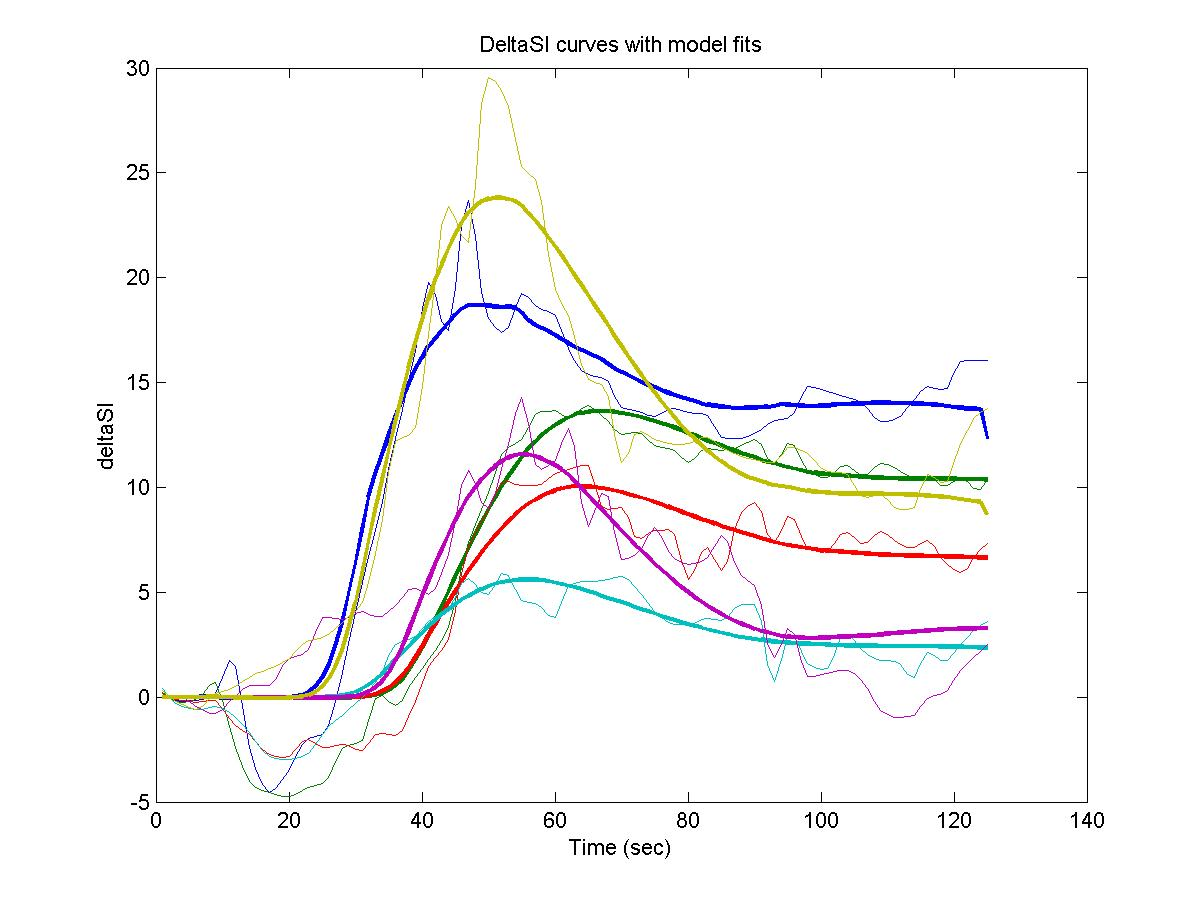
\includegraphics[width=17mm]{../Figures/Results_jpg_DZnomask/MoCo_07_DZNoMask_Rest_Fit.jpg} 
    \hspace{-5mm} &
    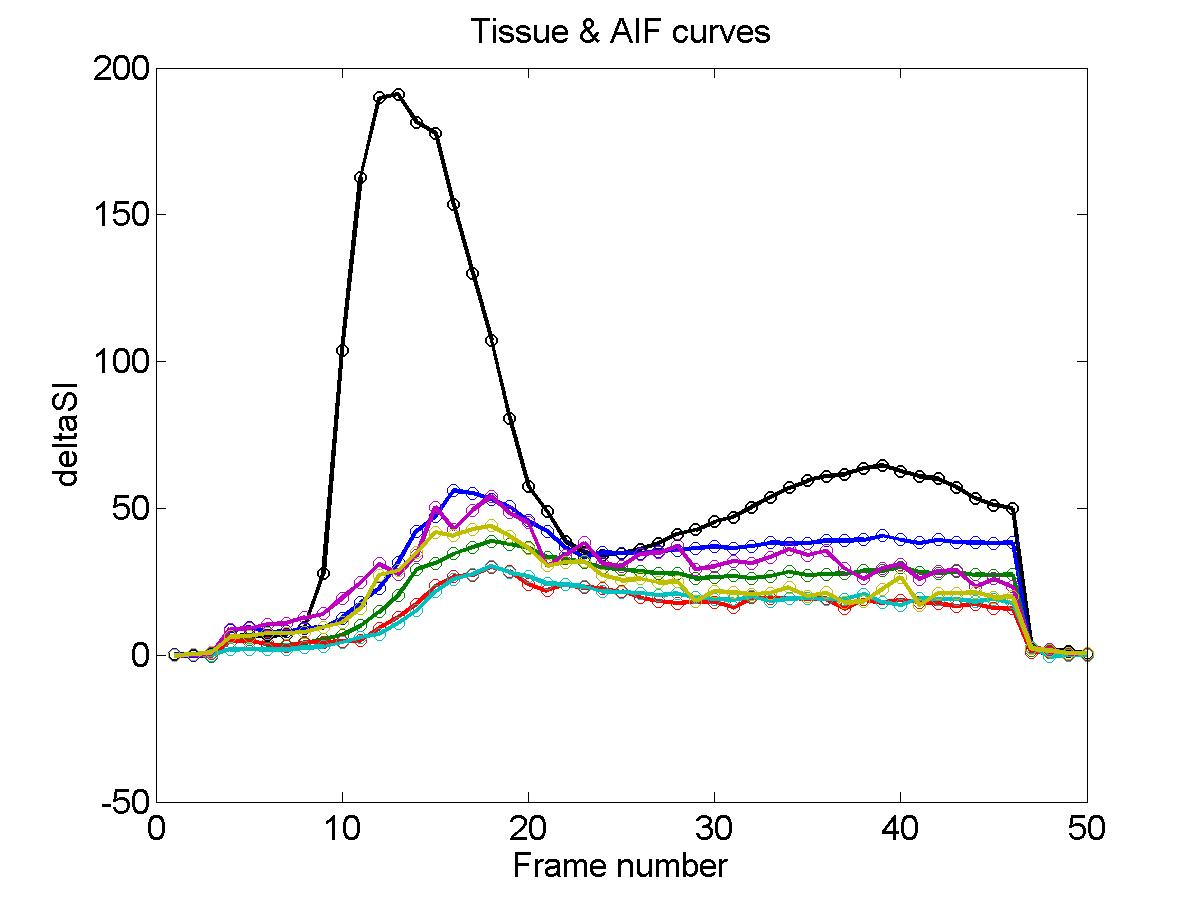
\includegraphics[width=17mm]{../Figures/Results_jpg_DZnomask/MoCo_07_DZNoMask_Stress_Curve.jpg} 
    \hspace{-5mm} &
    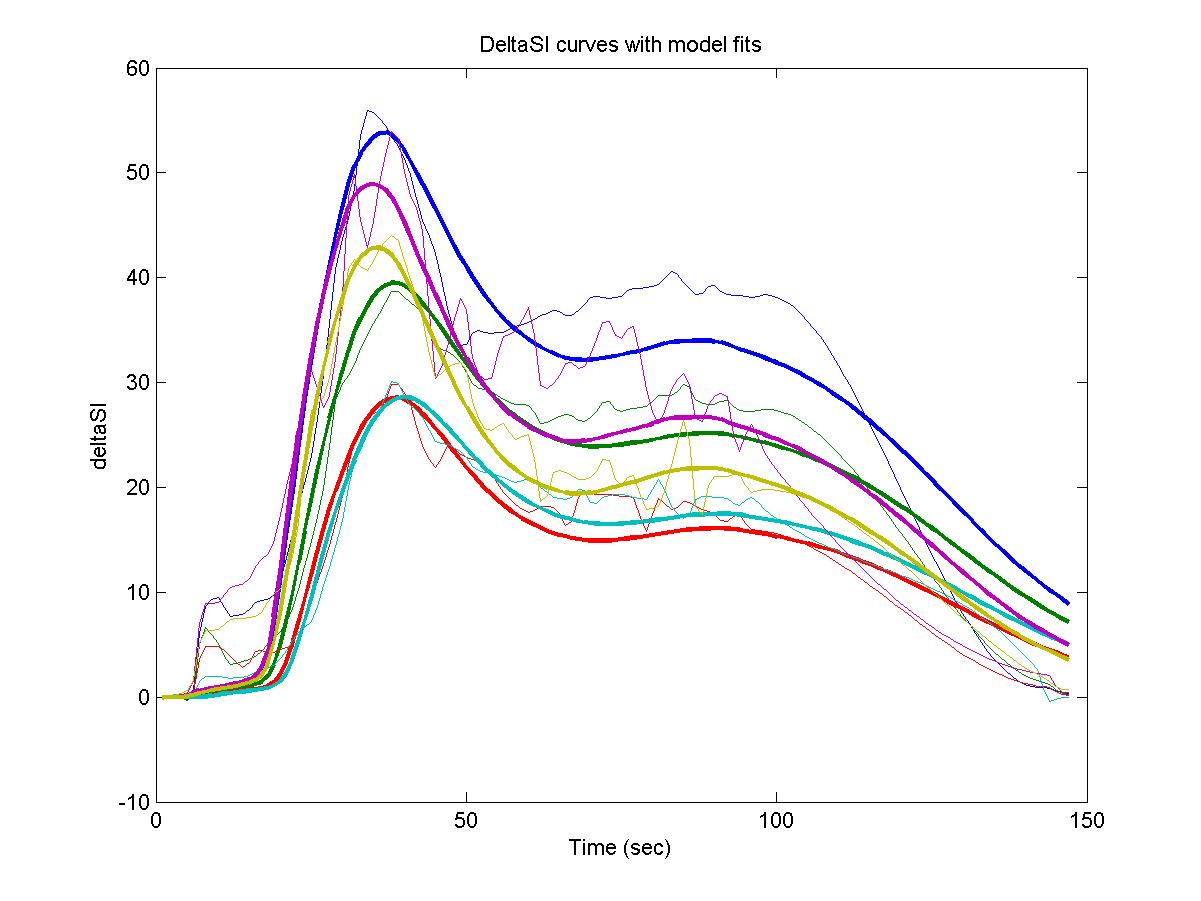
\includegraphics[width=17mm]{../Figures/Results_jpg_DZnomask/MoCo_07_DZNoMask_Stress_Fit.jpg} \\
    \rotatebox{90}{\tiny \bf\,\,\,\,\,\,\,MoCo\_08} & 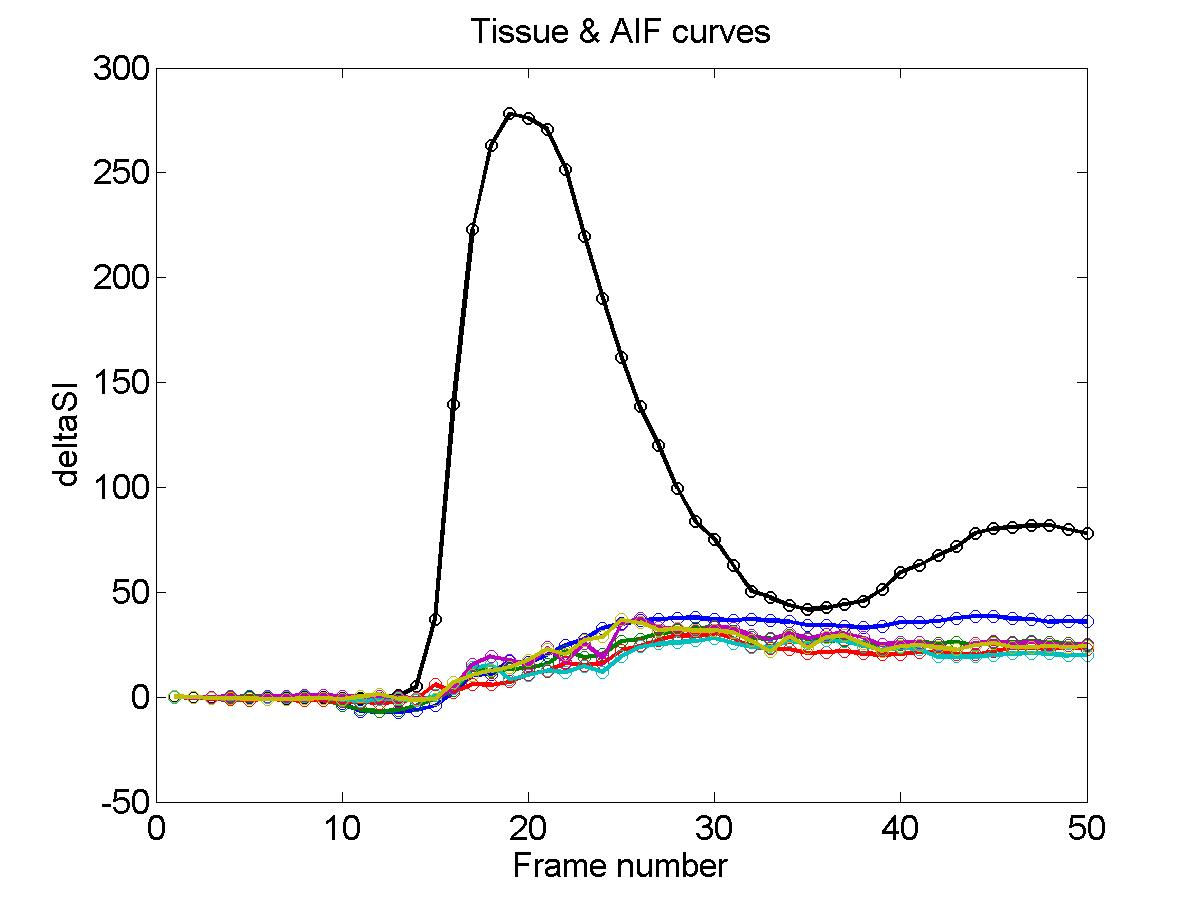
\includegraphics[width=17mm]{../Figures/Results_jpg_DZnomask/MoCo_08_DZNoMask_Rest_Curve.jpg} 
    \hspace{-5mm} &
    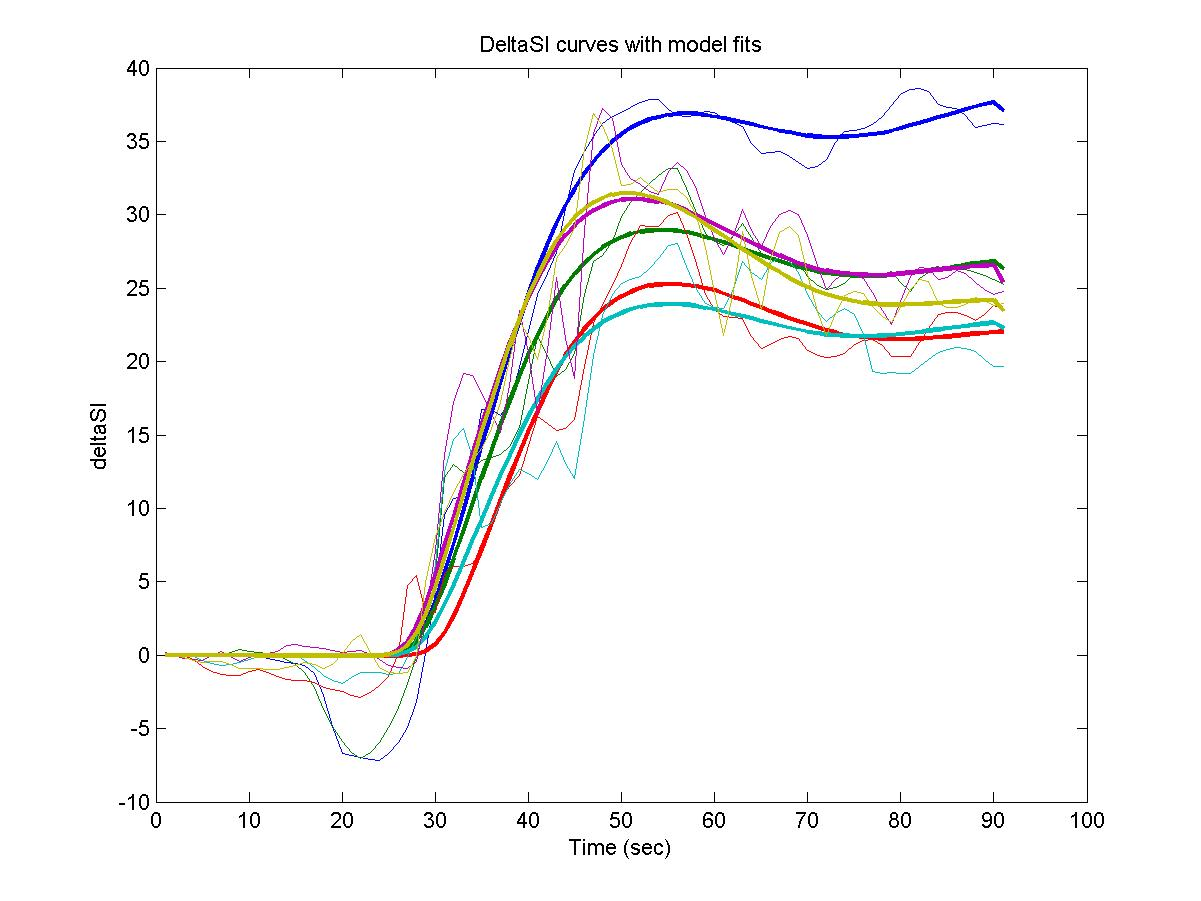
\includegraphics[width=17mm]{../Figures/Results_jpg_DZnomask/MoCo_08_DZNoMask_Rest_Fit.jpg} 
    \hspace{-5mm} &
    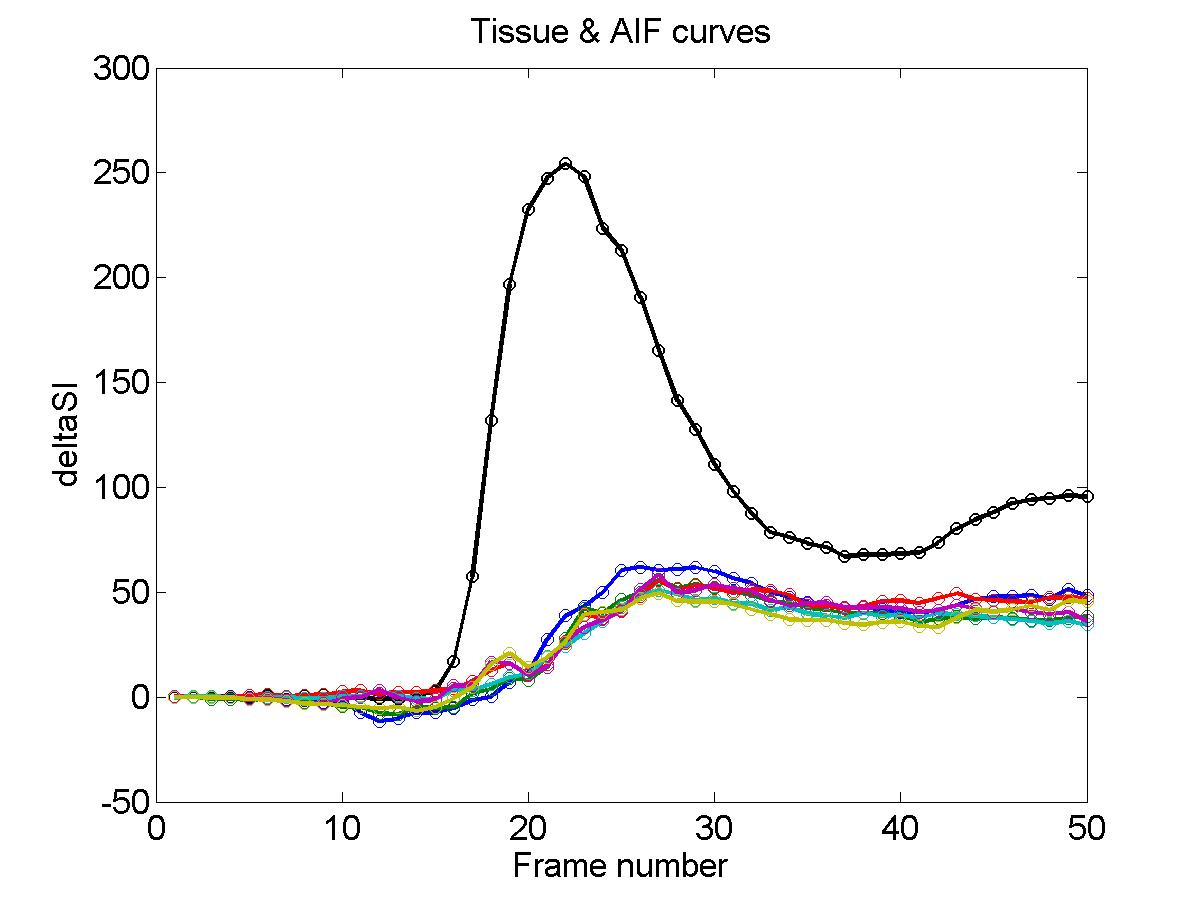
\includegraphics[width=17mm]{../Figures/Results_jpg_DZnomask/MoCo_08_DZNoMask_Stress_Curve.jpg} 
    \hspace{-5mm} &
    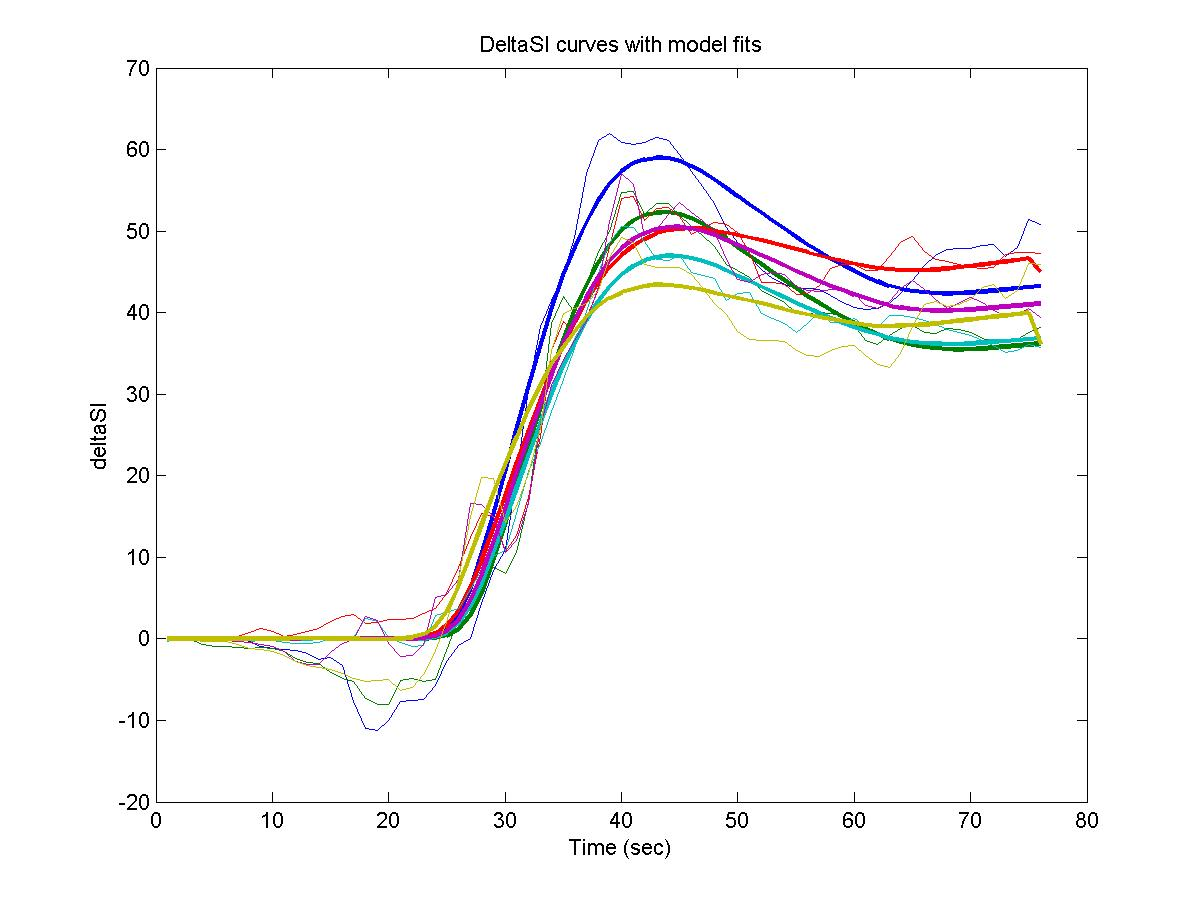
\includegraphics[width=17mm]{../Figures/Results_jpg_DZnomask/MoCo_08_DZNoMask_Stress_Fit.jpg} \\
    \rotatebox{90}{\tiny \bf\,\,\,\,\,\,\,MoCo\_09} & 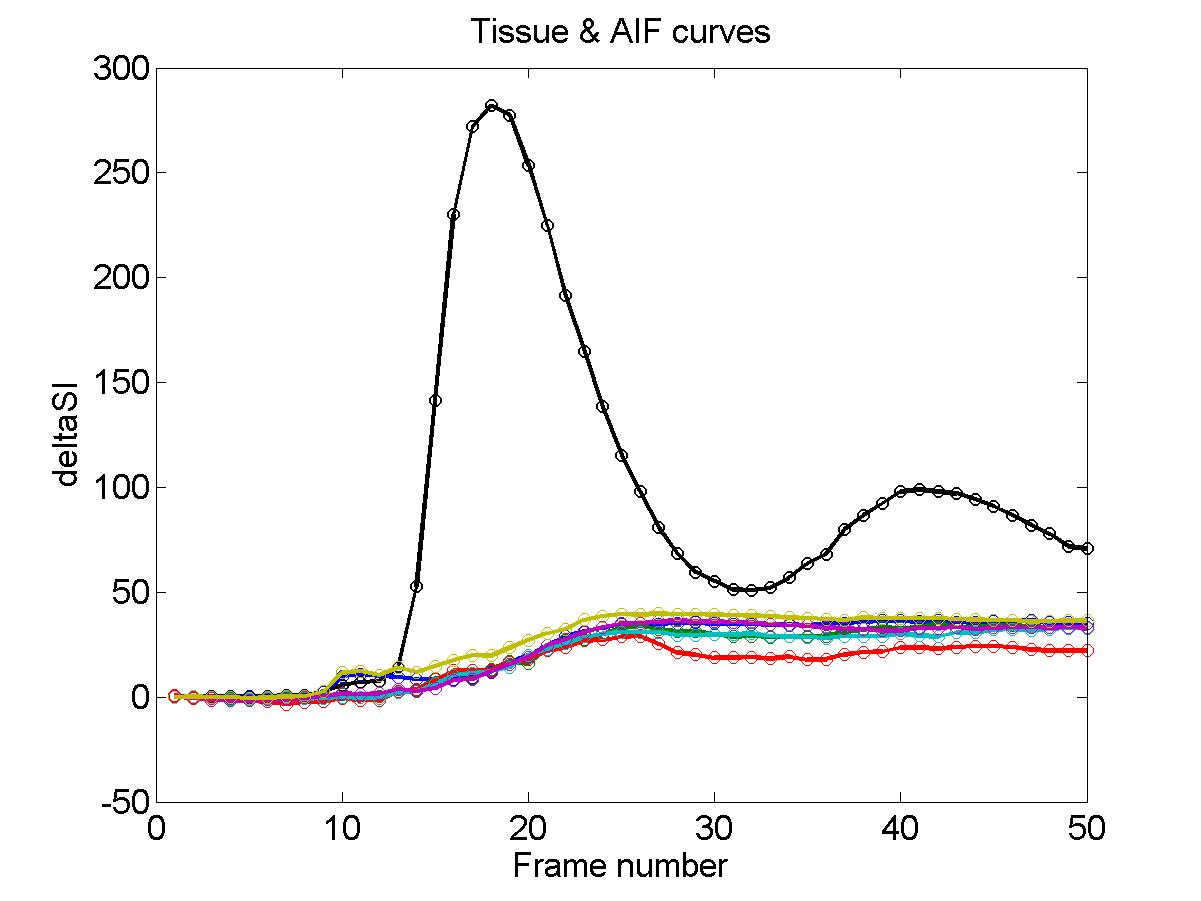
\includegraphics[width=17mm]{../Figures/Results_jpg_DZnomask/MoCo_09_DZNoMask_Rest_Curve.jpg} 
    \hspace{-5mm} &
    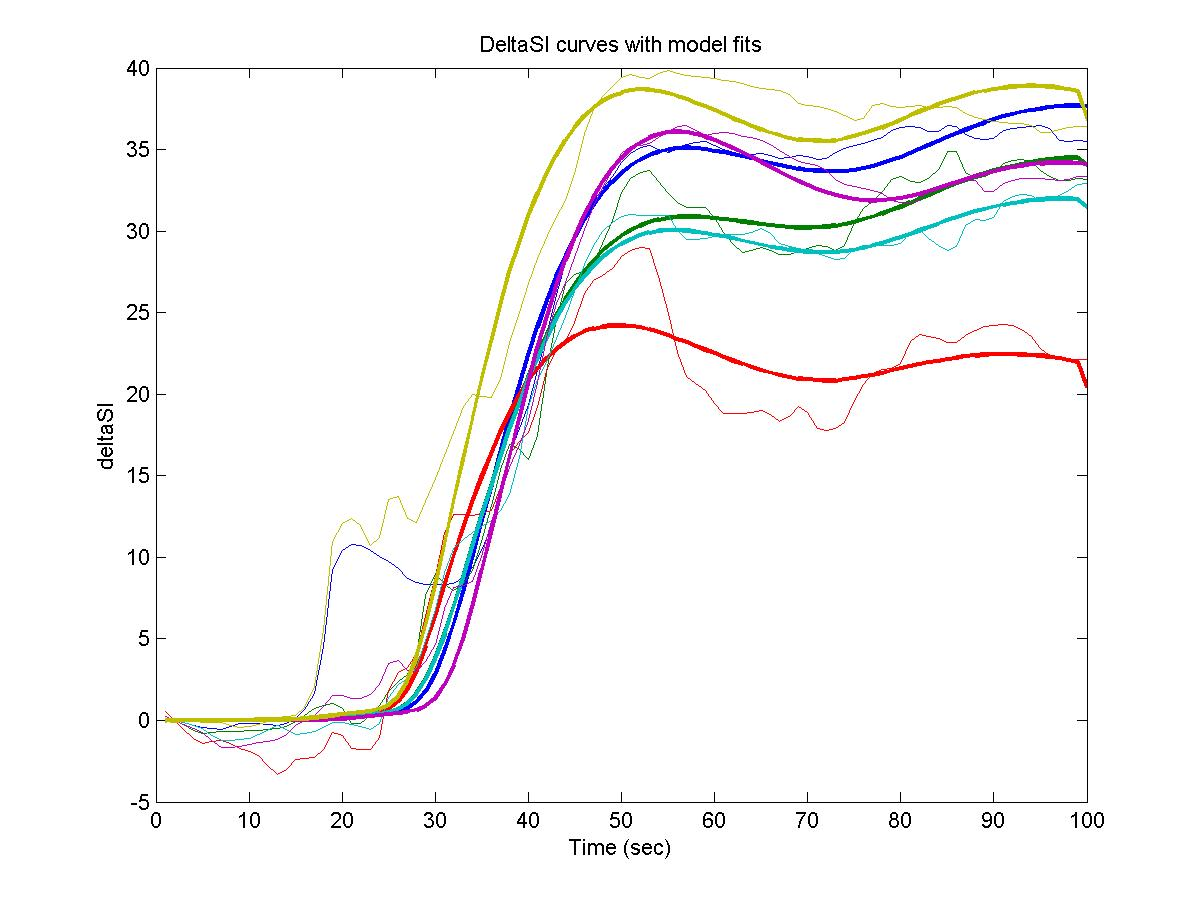
\includegraphics[width=17mm]{../Figures/Results_jpg_DZnomask/MoCo_09_DZNoMask_Rest_Fit.jpg} 
    \hspace{-5mm} &
    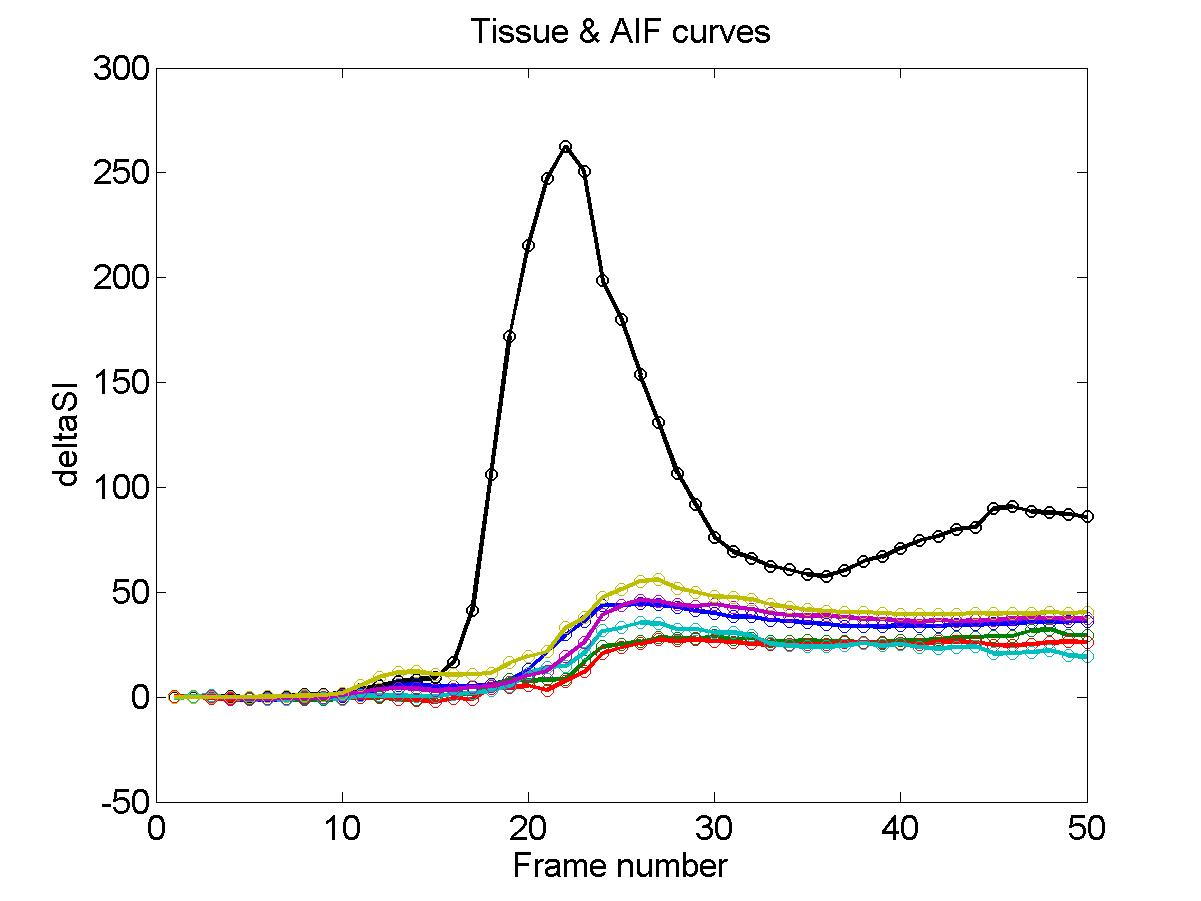
\includegraphics[width=17mm]{../Figures/Results_jpg_DZnomask/MoCo_09_DZNoMask_Stress_Curve.jpg} 
    \hspace{-5mm} &
    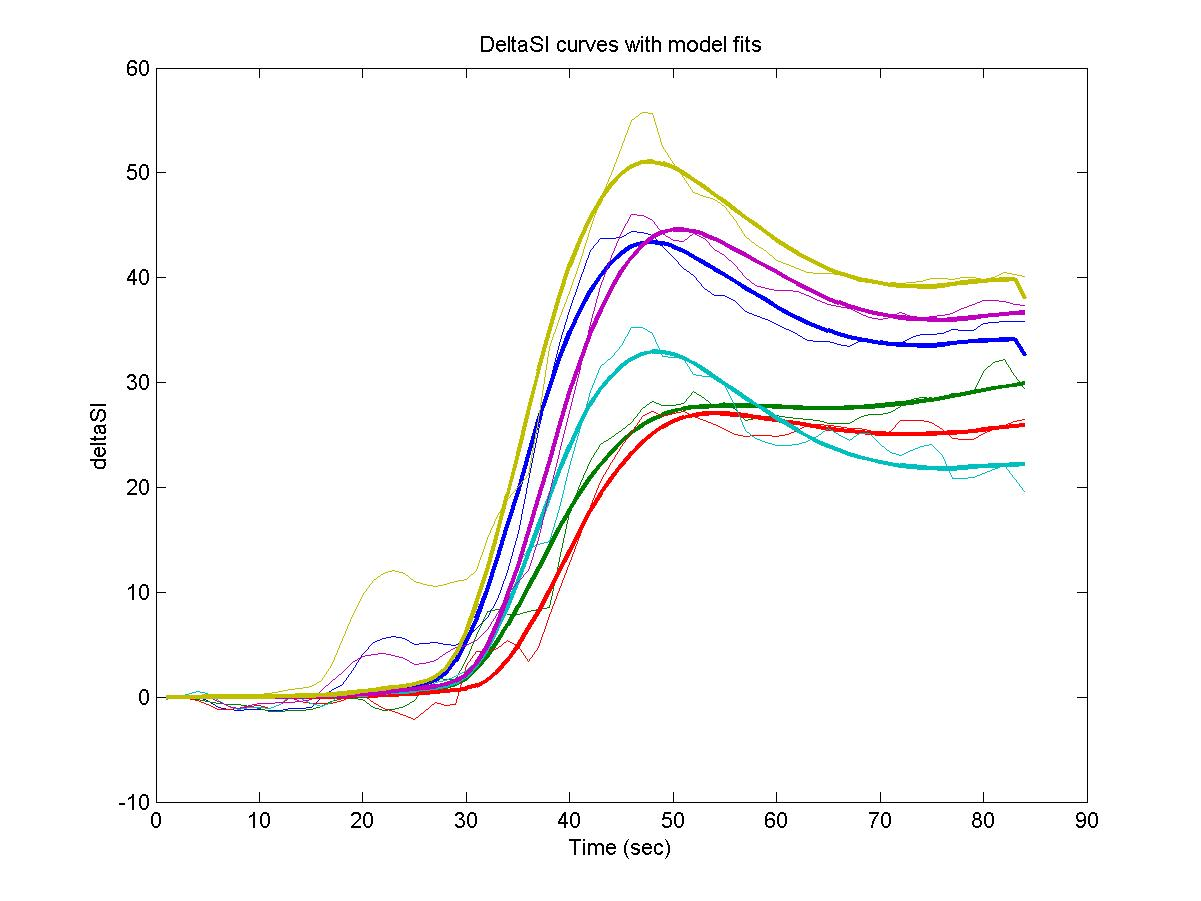
\includegraphics[width=17mm]{../Figures/Results_jpg_DZnomask/MoCo_09_DZNoMask_Stress_Fit.jpg} \\
    \rotatebox{90}{\tiny \bf\,\,\,\,\,\,\,MoCo\_10} & 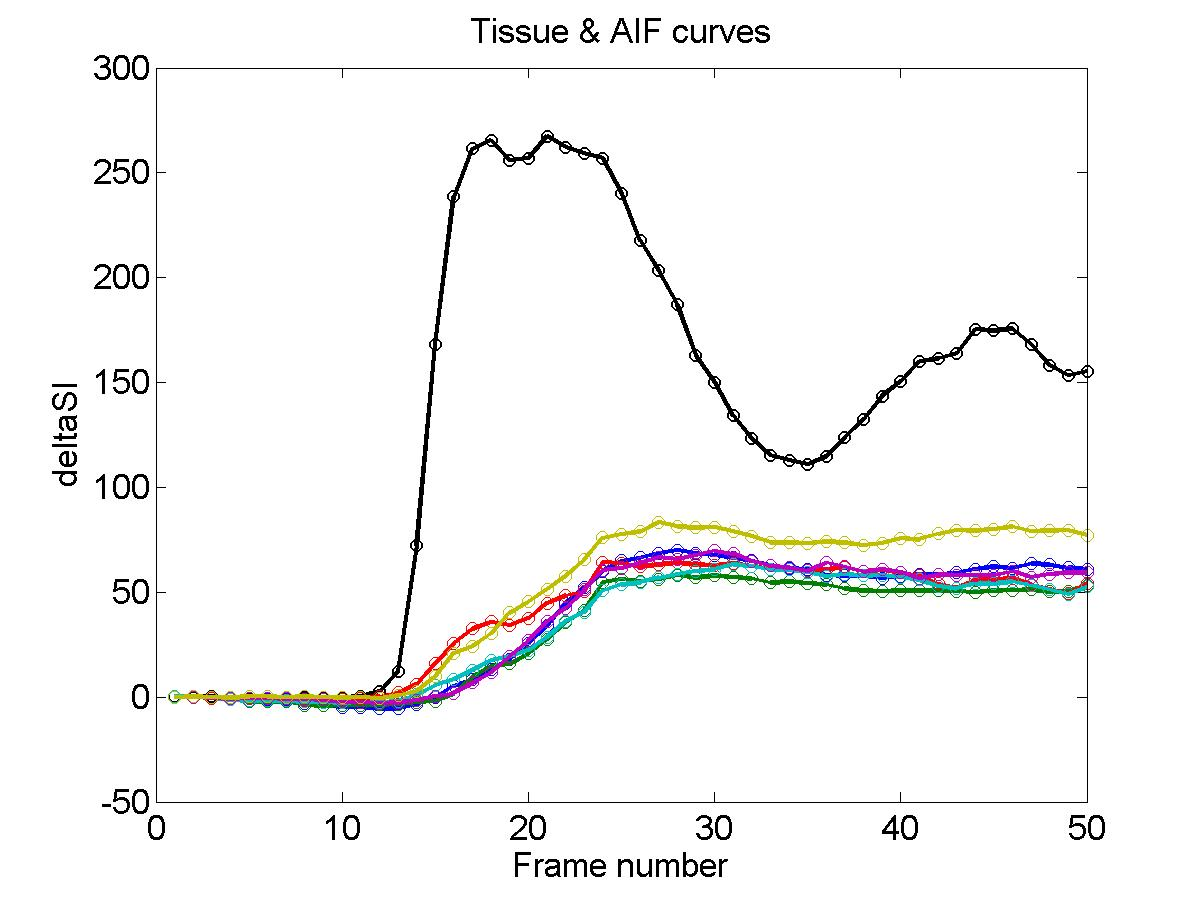
\includegraphics[width=17mm]{../Figures/Results_jpg_DZnomask/MoCo_10_DZNoMask_Rest_Curve.jpg} 
    \hspace{-5mm} &
    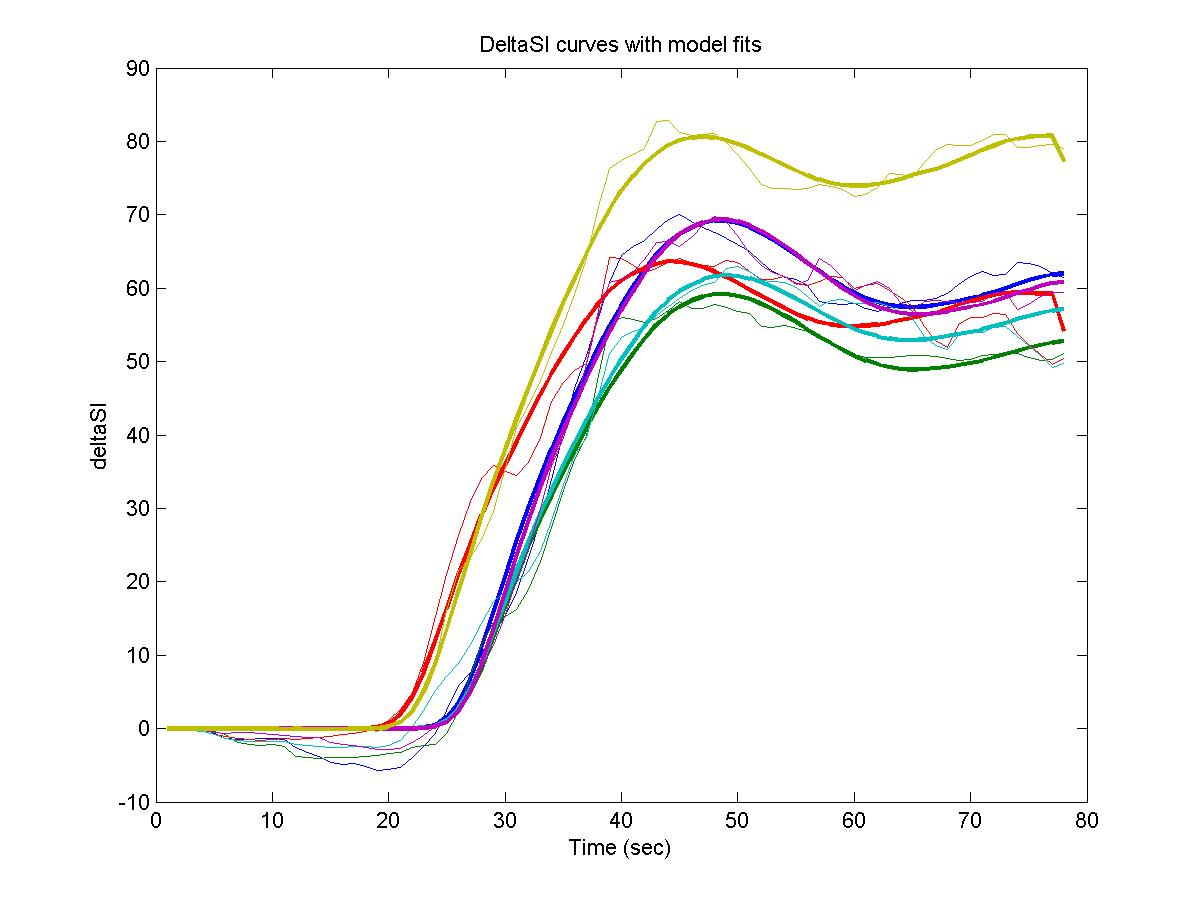
\includegraphics[width=17mm]{../Figures/Results_jpg_DZnomask/MoCo_10_DZNoMask_Rest_Fit.jpg} 
    \hspace{-5mm} &
    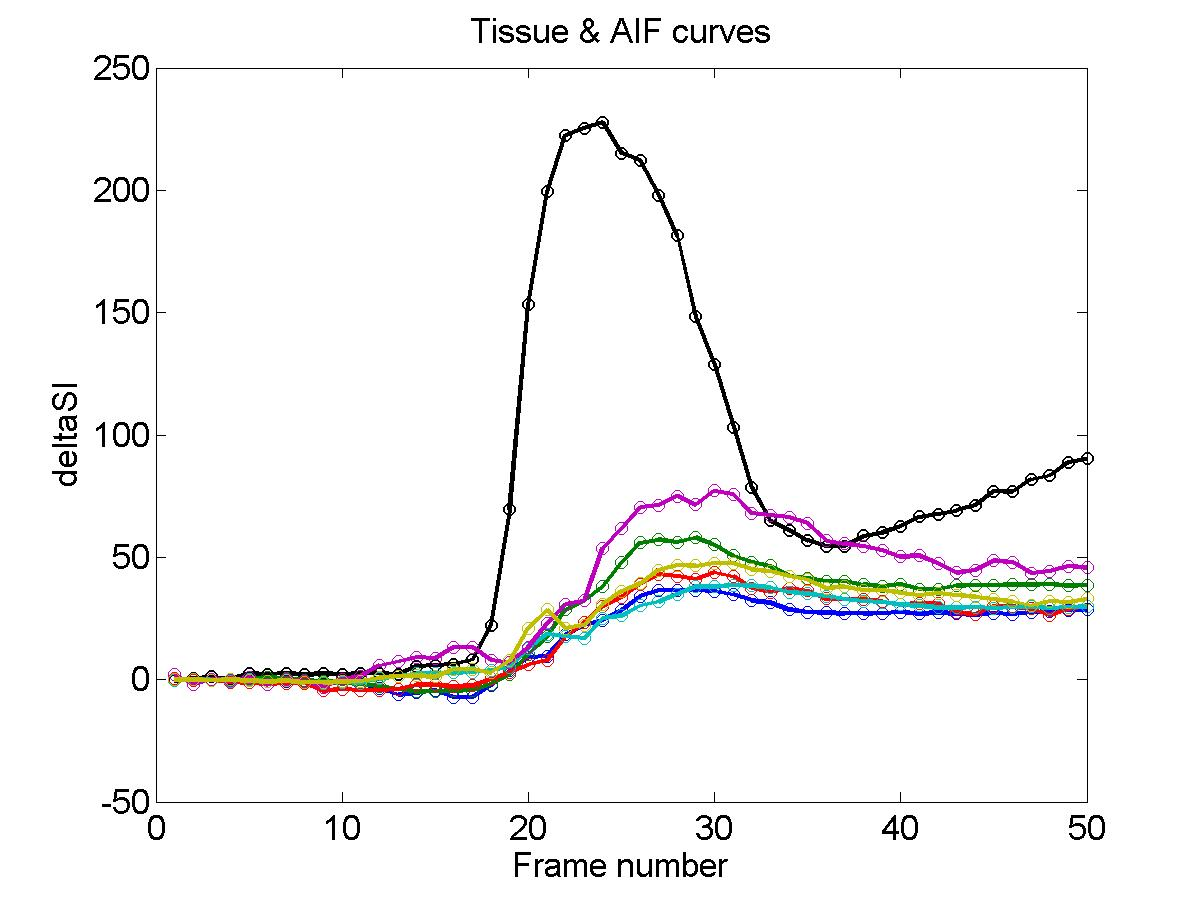
\includegraphics[width=17mm]{../Figures/Results_jpg_DZnomask/MoCo_10_DZNoMask_Stress_Curve.jpg} 
    \hspace{-5mm} &
    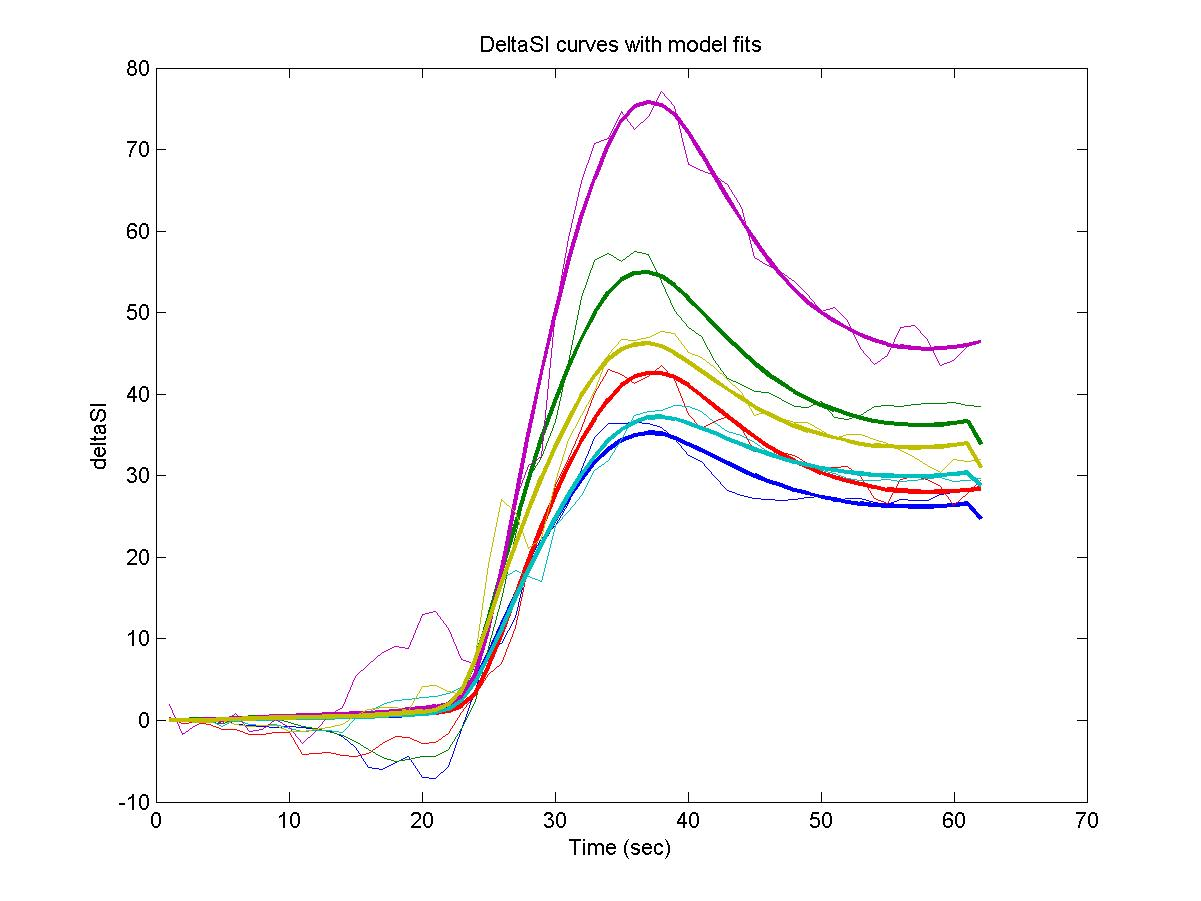
\includegraphics[width=17mm]{../Figures/Results_jpg_DZnomask/MoCo_10_DZNoMask_Stress_Fit.jpg} \\
    \rotatebox{90}{\tiny \bf \qquad Ungated} 
    & 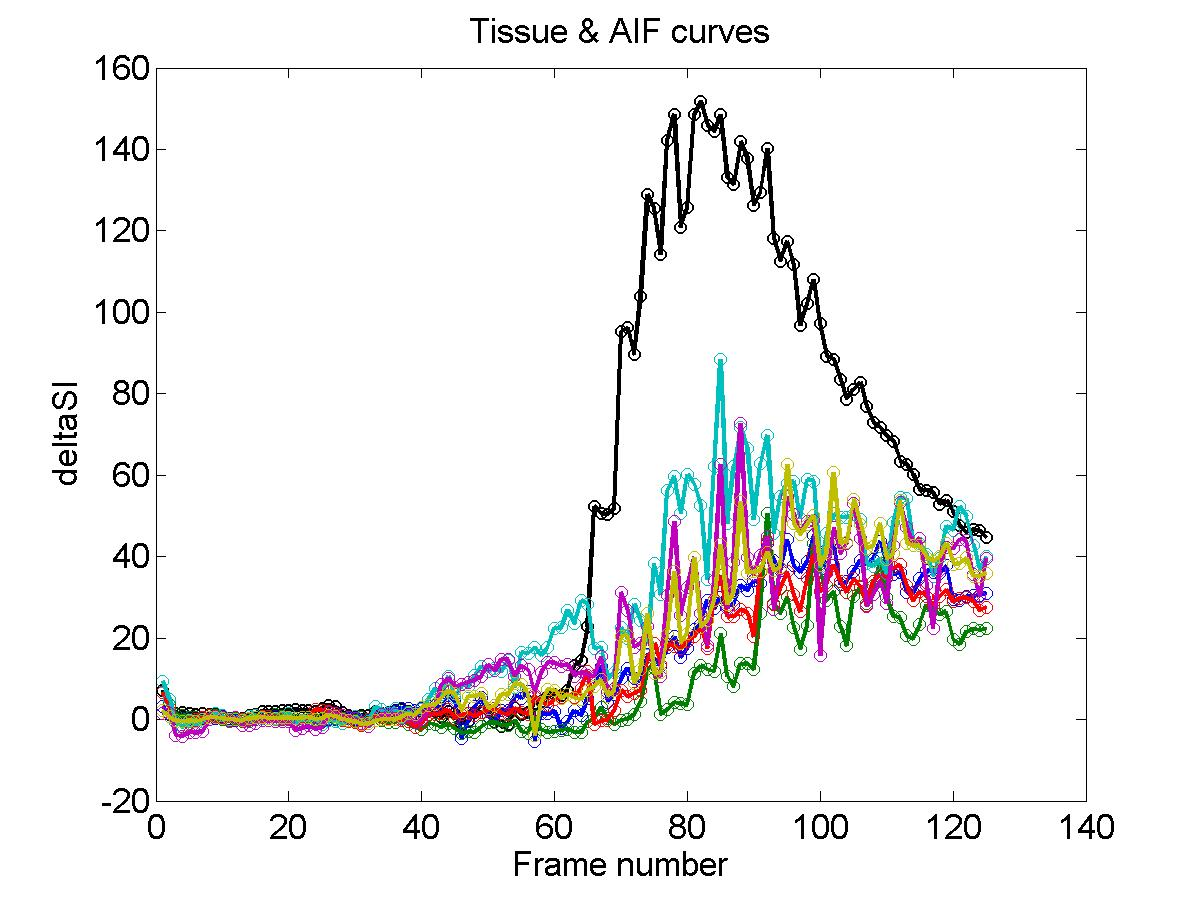
\includegraphics[width=17mm]{../Figures/Results_jpg_DZnomask/MoCo_Ungated_DZNoMask_Rest_Curve.jpg} 
    \hspace{-5mm} &
    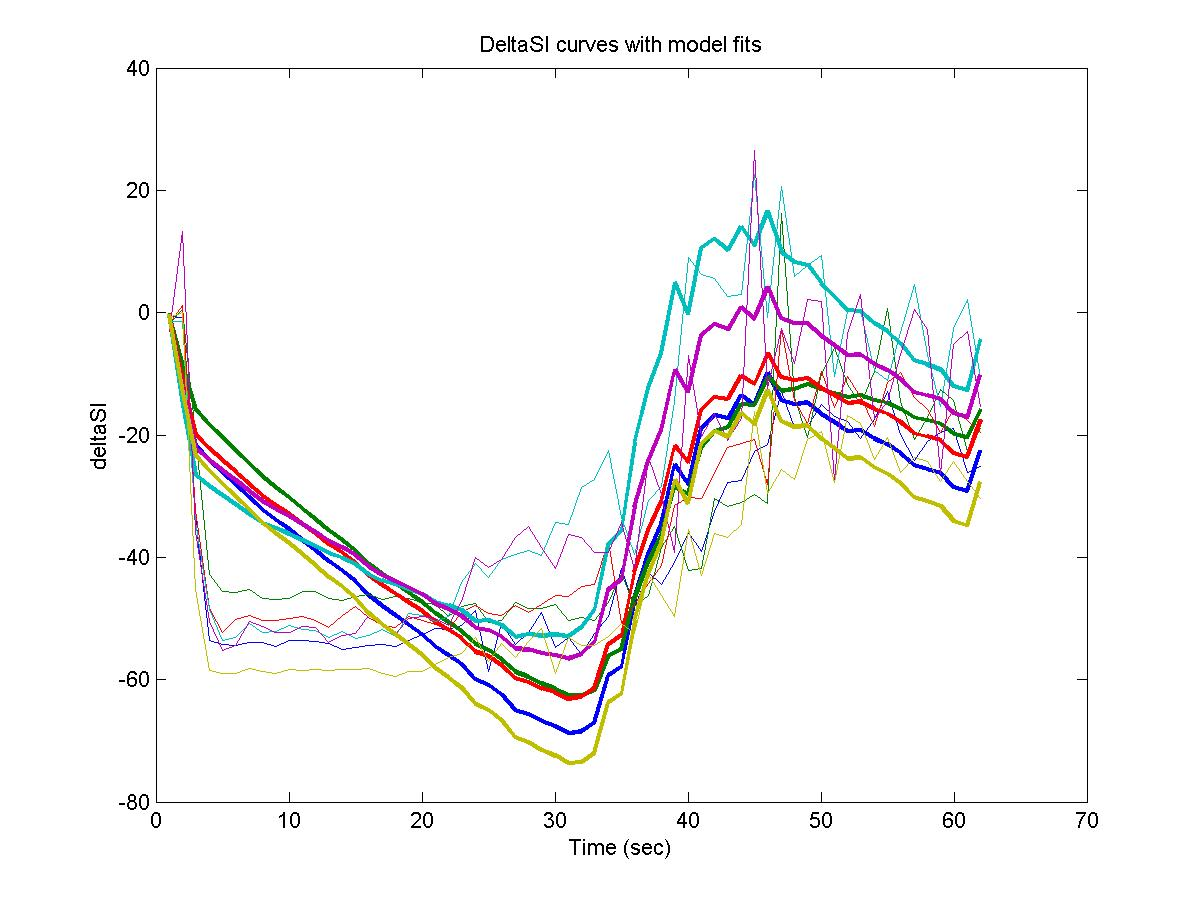
\includegraphics[width=17mm]{../Figures/Results_jpg_DZnomask/MoCo_Ungated_DZNoMask_Rest_Fit.jpg} 
    \hspace{-5mm} &
    {} & {}
  \end{tabular} 
  }
  
\end{center}

{\bf $K^{trans}$ values for all data for all 6 ROIs.}
\vspace{-0.3em}
{\tiny
\begin{center}
   \begin{tabular}{c d{4} d{4} d{4} d{4} d{4} d{4}}
    \toprule
	{} & \multicolumn{1}{c}{ROI$_1$} & \multicolumn{1}{c}{ROI$_2$} & 
	     \multicolumn{1}{c}{ROI$_3$} & \multicolumn{1}{c}{ROI$_4$} & 
	     \multicolumn{1}{c}{ROI$_5$} & \multicolumn{1}{c}{ROI$_6$} \\
	\midrule
	{\bf MoCo\_01} (rest) & 0.7646 & 0.793 & 0.6472 & 0.6223 & 1.1396 & 0.6169 \\
	{\bf MoCo\_01} (stress) & 2.991 & 3.3591 & 3.3946 & 3.8864 & 3.6427 & 2.9233 \\
	\midrule
	{\bf MoCo\_02} (rest) & 1.26 & 0.8393 & 0.8038 & 0.8026 & 0.621 & 0.9659 \\
	{\bf MoCo\_02} (stress) & 3.6184 & 4.7307 & 2.4689 & 2.1684 & 2.0884 & 4.6189 \\
	\midrule
	{\bf MoCo\_03} (rest) & 1.3238 & 1.0138 & 1.9537 & 1.4278 & 0.6698 & 1.2323 \\
	{\bf MoCo\_03} (stress) & 4.6317 & 4.482 & 2.5719 & 2.2236 & 1.2169 & 3.3639 \\
	\midrule
	{\bf MoCo\_04} (rest) & 2.4826 & 1.958 & 1.7667 & 2.0848 & 3.0735 & 2.516 \\
	{\bf MoCo\_04} (stress) & 6.6083 & 10.1963 & 9.2774 & 10.0296 & 10.7357 & 8.875 \\
	\midrule
	{\bf MoCo\_05} (rest) & 1.6678 & 1.4952 & 0.8095 & 0.8683 & 1.1663 & 1.318\\
	{\bf MoCo\_05} (stress) & 2.4283 & 2.6987 & 2.0908 & 1.9775 & 2.3872 & 3.0467 \\
	\midrule
	{\bf MoCo\_06} (rest) & 0.9946 & 1.2878 & 1.1367 & 0.7262 & 0.8156 & 0.865\\
	{\bf MoCo\_06} (stress) & 2.1543 & 2.6292 & 2.1322 & 2.59 & 1.4002 & 1.4648 \\
	\midrule
	{\bf MoCo\_07} (rest) & 0.6009 & 0.5397 & 0.4214 & 0.2904 & 0.8107 & 1.234\\
	{\bf MoCo\_07} (stress) & 2.8381 & 2.2815 & 1.8141 & 1.7029 & 2.7065 & 2.8503 \\
	\midrule
	{\bf MoCo\_08} (rest) & 1.0315 & 0.8754 & 0.7959 & 0.7106 & 0.9726 & 1.0769 \\
	{\bf MoCo\_08} (stress) & 3.1103 & 2.9066 & 2.2222 & 2.369 & 2.4781 & 1.796 \\
	\midrule
	{\bf MoCo\_09} (rest) & 1.0073 & 0.8589 & 0.7194 & 0.8689 & 1.1375 & 1.1258 \\
	{\bf MoCo\_09} (stress) & 1.939 & 0.9883 & 1.0515 & 1.6527 & 1.9416 & 2.2943 \\
	\midrule
	{\bf MoCo\_10} (rest) & 2.734 & 2.3579 & 2.2832 & 2.3316 & 2.822 & 2.743\\
	{\bf MoCo\_10} (stress) & 2.2161 & 3.8051 & 2.9618 & 2.234 & 5.6507 & 2.9052 \\
	\midrule
	{\bf Ungated} &	2.3471 & 3.0672 & 2.6664 & 3.7773 &	3.5338 & 2.7093 \\
	\bottomrule
  \end{tabular}\end{center}
}
}


%%%%%%%%%%%%%%%%%%%%%%%%%%%%%%%%%%%%%%%%%%%%%%%%%%%%%%%%%%%%%%%%%%%%%%%%%%%%%%
%  \headerbox{Conclusions}{name=conclusions,column=1,below=results}{
%%%%%%%%%%%%%%%%%%%%%%%%%%%%%%%%%%%%%%%%%%%%%%%%%%%%%%%%%%%%%%%%%%%%%%%%%%%%%%
%
% SCCA demonstrates significant differences between the control and patient groups in both the FA ($p < 0.002$) and gray matter ($p < 0.04$)	that	are	widespread 	but	largely	focus	on	 thalamocortical networks related to the limbic system. Specific regional differences included the medial thalamic nuclei, hypothalamus, amygdala, hippocampus, anterior cingulate cortex, orbitofrontal cortex and fornix. Using these SCCA-identified regions, we demonstrate a strong correlation ($p < 0.01$) of the degree of injury in WM and GM within the patient group.
% 
%\vspace{0.3em}
%  }
%
%%%%%%%%%%%%%%%%%%%%%%%%%%%%%%%%%%%%%%%%%%%%%%%%%%%%%%%%%%%%%%%%%%%%%%%%%%%%%
  \headerbox{References}{name=references,column=2,below=evaluation,above=bottom}{
%%%%%%%%%%%%%%%%%%%%%%%%%%%%%%%%%%%%%%%%%%%%%%%%%%%%%%%%%%%%%%%%%%%%%%%%%%%%%

\vspace{2mm}
    \tiny % \scriptsize
      \vspace{-0.4em}
      \renewcommand{\refname}{\vspace{-0.8em}}
      \bibliographystyle{abbrv}
      \bibliography{../references}



%    \bibliographystyle{ieee}
%    \renewcommand{\section}[2]{\vskip 0.05em}
%      \begin{thebibliography}{1}\itemsep=-0.01em
%      \setlength{\baselineskip}{0.4em}
%      \bibitem{amberg07:nonrigid}
%        B.~Amberg, S.~Romdhani, T. Vetter.
%        \newblock {O}ptimal {S}tep {N}onrigid {ICP} {A}lgorithms for {S}urface {R}egistration
%        \newblock In {\em Computer Vision and Pattern Recognition 2007}
%      \bibitem{amberg08:recognition}
%        B.~Amberg, R.~Knothe, T. Vetter.
%        \newblock Expression Invariant Face Recognition with a 3D Morphable Model
%        \newblock In {\em Automated Face and Gesture Recognition 2008}
%      \end{thebibliography}
  }


%%%%%%%%%%%%%%%%%%%%%%%%%%%%%%%%%%%%%%%%%%%%%%%%%%%%%%%%%%%%%%%%%%%%%%%%%%%%%%
%  \headerbox{Acknowledgments}{name=acknowledgments,column=1,below=conclusions,above=bottom}{
%%%%%%%%%%%%%%%%%%%%%%%%%%%%%%%%%%%%%%%%%%%%%%%%%%%%%%%%%%%%%%%%%%%%%%%%%%%%%%
%  \vspace{1mm}
%  \smaller
%   This is my acknowledgment.
%  }

%%%%%%%%%%%%%%%%%%%%%%%%%%%%%%%%%%%%%%%%%%%%%%%%%%%%%%%%%%%%%%%%%%%%%%%%%%%%%%%
%  \headerbox{Expression Neutralization}{name=results neutralization,column=1,row=0}{
%%%%%%%%%%%%%%%%%%%%%%%%%%%%%%%%%%%%%%%%%%%%%%%%%%%%%%%%%%%%%%%%%%%%%%%%%%%%%%%
%  \begin{tikzpicture}[x=0.3333\linewidth,y=-0.42\linewidth]
%    \path [use as bounding box] (-0.5,-0.5) rectangle(2.5,1.7);
%    \path
%    (0,0) node{\includegraphics[width=0.42\linewidth]{D1077}}
%    (1,0) node{\includegraphics[width=0.47\linewidth]{D1077_fit_expression}}
%    (2,0) node{\includegraphics[width=0.47\linewidth]{D1077_fit}}
%
%    (0,1) node{\includegraphics[width=0.42\linewidth]{D1360}}
%    (1,1) node{\includegraphics[width=0.47\linewidth]{D1360_fit_expression}}
%    (2,1) node{\includegraphics[width=0.47\linewidth]{D1360_fit}}
%
%    (0,1.6) node {\smaller a) Target}
%    (1,1.6) node {\smaller b) Fit}
%    (2,1.6) node {\smaller c) Normalized};
%  \end{tikzpicture}
%  \vspace{0.5em}
%
%  Expression normalisation for two scans of the same individual.  
%  The robust fitting gives a good estimate (b) of the true face surface given
%  the noisy measurement (a). It fills in holes and removes artifacts using
%  prior knowledge from the face model. The pose and expression normalized faces
%  (c) are used for face recognition.
%  \vspace{0.5em}
%  }
%%%%%%%%%%%%%%%%%%%%%%%%%%%%%%%%%%%%%%%%%%%%%%%%%%%%%%%%%%%%%%%%%%%%%%%%%%%%%%%
%  \headerbox{Funding}{name=funding,column=1,span=2,above=bottom}{
%%%%%%%%%%%%%%%%%%%%%%%%%%%%%%%%%%%%%%%%%%%%%%%%%%%%%%%%%%%%%%%%%%%%%%%%%%%%%%%
%  \smaller 
%  \hspace{1em}This work was supported in part by Microsoft Research through the European PhD Scholarship Programme.
%  }
%%%%%%%%%%%%%%%%%%%%%%%%%%%%%%%%%%%%%%%%%%%%%%%%%%%%%%%%%%%%%%%%%%%%%%%%%%%%%%%
%  \headerbox{Robustness}{name=robustness,column=2,row=0,above=results,span=1}{
%%%%%%%%%%%%%%%%%%%%%%%%%%%%%%%%%%%%%%%%%%%%%%%%%%%%%%%%%%%%%%%%%%%%%%%%%%%%%%%
%  \begin{tikzpicture}[x=0.3333\linewidth,y=-0.42\linewidth]
%    \path [use as bounding box] (-0.5,-0.5) rectangle(2.5,1.7);
%    \path
%    (0,0) node{\includegraphics[width=0.42\linewidth]{D1160}}
%    (1,0) node{\includegraphics[width=0.42\linewidth]{D1425}}
%    (2,0) node{\includegraphics[width=0.42\linewidth]{D1205}}
%
%    (0,1) node{\includegraphics[width=0.28\linewidth]{D1160_fit_expression}}
%    (1,1) node{\includegraphics[width=0.28\linewidth]{D1425_fit_expression}}
%    (2,1) node{\includegraphics[width=0.28\linewidth]{D1205_fit_expression}}
%
%    (1,0.5) node {\smaller a) Target}
%    (1,1.6) node {\smaller b) Robust Reconstruction};
%  \end{tikzpicture}
%  \vspace{0.5em}
%
%  The reconstruction (b) is robust against scans (a) with artifacts, noise, and
%  holes.
%  
%  This is achieved by a robust iteratively reweighted ICP algorithm and outlier
%  rejection based on angle comparisions between corresponding points.
%  }


\end{poster}

\end{document}
